\documentclass[12pt]{ociamthesis}  % default square logo 
% \documentclass[12pt,beltcrest]{ociamthesis} % use old belt crest logo
%\documentclass[12pt,shieldcrest]{ociamthesis} % use older shield crest logo

%load any additional packages

% ---- START OF CUSTOM CONFIGURATION ----

\usepackage{amssymb} % unknown
\usepackage{array} % unknown
\usepackage{courier} % give courier font to listings and also \texttt{}
\usepackage{xcolor} % add colors to text using \textcolor{red}{<text>}
\usepackage{amsmath} % unknown
\usepackage{ulem} % unknown
\usepackage{hyperref} % ability to add links using \href{<link>}{<label>}, also ability to make the contents page clickable
\usepackage{listings} % ability to print code using \begin{lstlisting}
\usepackage{graphicx} % ability to add image
\usepackage{tablefootnote} % ability to use table footnotes in table using command \tablefootnotes
\usepackage{multirow} % ability to merge rows using \mergerow
\usepackage{makecell} % ability to have line breaks inside tables
\usepackage{imakeidx} % add an index for the document
\makeindex % add an index for the document
% configure hyperref, display the contents page as its usual black color
\hypersetup{ 
    colorlinks,
    citecolor=black,
    filecolor=black,
    linkcolor=black,
    urlcolor=black
}

% configure listings
\lstset{language=C++}
\lstset{basicstyle=\ttfamily,breaklines=true} %use courier as font, also make sure it skips to another line when the text is too long for one line

\setlength{\parindent}{0pt} % disable indent of first line of each paragraph
\graphicspath{ {./images/} } % configure graphicx

% ---- END OF CUSTOM CONFIGURATION ----

%input macros (i.e. write your own macros file called mymacros.tex 
%and uncomment the next line)
%\include{mymacros}

\title{Intermediate Programming (DRAFT) %your thesis title,
        }   %note \\[1ex] is a line break in the title

\author{Oscar Mui }             %your name
\college{University College}  %your college

% \renewcommand{Notes for}{change the default text here if needed}
\degree{Computer Science \\[1ex] HKOI Training (in C++)}     %the degree
\degreedate{September 2022}         %the degree date

%end the preamble and start the document
\begin{document}

%this baselineskip gives sufficient line spacing for an examiner to easily
%markup the thesis with comments
\baselineskip=18pt plus1pt

%set the number of sectioning levels that get number and appear in the contents
\setcounter{secnumdepth}{3}
\setcounter{tocdepth}{3}


\maketitle                  % create a title page from the preamble info
\include{dedication}        % include a dedication.tex file
\include{acknowlegements}   % include an acknowledgements.tex file
\chapter*{Preface}

This piece of notes is originally made for students who are going to join the Hong Kong Olympiad in Informatics (HKOI). It covers some topics in the \link{https://hkoi.org/en/competition-syllabus/}{HKOI syllabus} that I found the most useful. Aiming to introduce senior secondary school (high school) students with more advanced programming theories, so as to prepare them for competitive programming competitions like HKOI. 

At the same time, it also serves as a good revision material for students taking public examination on programming, such as HKDSE ICT and IB Computer Science. However, it is highly likely that not everything in the syllabus is covered. Some advanced contents are included, especially in the exercises, to enlighten students who aim to study Computer Science in university. 

The name of this piece of notes is ``Intermediate Programming'', so I expect readers to have basic knowledge in programming, including if statements, variables, loops, arrays and functions, in any programming language. However, we will still briefly go through them in \cref{sec:elementary} as a recap and for you to familiarise yourself with the C++ syntax.

It is a simplified piece of notes with a huge number of links to other resources, as the internet is a better teacher than me, yet I am here to provide you with information that I found the most useful when I was in your position a few years ago.

The source code of this notes can be found on \link{https://github.com/OscarMui/Intermediate-Programming-Notes}{GitHub}.

\section*{About me}

I am a third-year undergraduate student studying Computer Science at the University of Oxford, United Kingdom. I joined the senior group HKOI before in the year 2020-2021 and obtained a silver award at the finals. 

\section*{Choice of programming language}
I would like to stress that the choice of programming language is an arbitrary one (that is helpful for those doing the HKOI competition). Most of the concepts in this piece of notes apply to other programming languages such as Java, C and Python.

\section*{A word of warning}

This piece of notes aims to include everything in the shortest amount of time possible, so explanations and examples may be inadequate. Unfortunately, a small amount of sections of the notes are incomplete due to a lack of time, you should be able to fill in the gaps on your own by asking Google.

The fact that it serves multiple parties means that some of the sections may not be at a suitable difficulty. The \textit{Difficult topic}, \textit{Of less importance} and \textit{Out of scope} labels may help. Readers should consult their instructors when they are not sure which parts they should skip, or which exercises they should do.

Note that questions with wordings like ``Discuss with your instructor'' are open ended so there will not be an absolute correct answer.

          % include the abstract

\begin{romanpages}          % start roman page numbering
\tableofcontents            % generate and include a table of contents
% \listoffigures              % generate and include a list of figures
\end{romanpages}            % end roman page numbering

%now include the files of latex for each of the chapters etc
\chapter{Hong Kong Olympiad in Informatics}

Even though the knowledge you will take away by joining the competition is more important than specific skills related to the competition, I think it is still worth it to mention the key points.

\section{About the competition}
\textit{IMPORTANT: rules of HKOI might have changed over the years, please refer to the \href{https://hkoi.org/en/}{HKOI website}\footnote{Link: \href{https://hkoi.org/en/}{https://hkoi.org/en/}} for the latest rules.}
\vspace{6mm}

The competition is split into Junior Group and Senior Group, you would need to be born after a certain date in order to join the Junior Group. (usually S5 students or above have to join the Senior Group, but some lucky ones are young enough for the Junior Group, seize this opportunity if this is your case)
\vspace{6mm}

The competition consists of two parts, heats and finals.
\vspace{6mm}

The heat event is usually held in November, a 1.5-hour written test. Junior Group contestants are given 5 True or False questions, 20 MC questions (each worth 1 mark each), and 20 marks worth of Short Questions. Senior Group contestants are given 25 MC questions (each worth 1 mark each), and 20 marks worth of Short Questions. Making the total score 45. 

There are only two grades you can get in the heats, that is, PASS or FAIL. The mark you get in heats will not affect your award in the finals, The passing mark fluctuates so that around 100 contestants enter the finals. The passing mark of previous years can be found in the \href{https://hkoi.org/en/past-problems/}{official solution of the heat event}.\footnote{Link: \href{https://hkoi.org/en/past-problems/}{https://hkoi.org/en/past-problems/}}
\vspace{6mm}

The final event is usually held in December, a 3-hour practical test. Where you write code to solve 4 problems, each worth 100 marks, bringing the total to 400. Prizes will be given based on the total mark you get out of 400.
\vspace{6mm}

The best programming language for both the heats and finals in my opinion is C++.
\vspace{6mm}

Regardless of your final result, this is a good experience and a good opportunity to learn more about computing, I hope all of you would enjoy it.

\section{General tips on heats}
\begin{enumerate}
    \item Don't be too stressed out, it is fine as long as you get a higher score than the cutoff.
    \item Answer every MC question, make guesses if you are not sure.
    \item Remember basic C++ syntax so that you know the shortest way to write the code needed for the short questions, as there are character limits imposed on your answers. (see the answer sheet of the heat event)
\end{enumerate}

\section{General tips on finals}
\begin{enumerate}
    \item Focus on the first few subtasks of each question. They are usually easier, and you will be able to at least get some of the marks.
    \item Note that you will only get the marks for the subtask when you pass ALL the test cases.
    \item Remember basic C++ syntax to reduce thinking time.
\end{enumerate}
% Translated to Java

\if\proglang1
\chapter{Java Knowledge}
\else
\chapter{C++ Knowledge}
\fi


Here are some basic\if\proglang1 Java \else ~C++ \fi knowledge, I bet you have seen some of the concepts in this chapter already on other occasions.

% Translated to Java end 

\section{Further resources (Ch 2-3)}
\href{https://www.youtube.com/watch?v=tvC1WCdV1XU&list=PLAE85DE8440AA6B83}{Bucky's C++ Programming Tutorial}\footnote{Link: \href{https://www.youtube.com/watch?v=tvC1WCdV1XU&list=PLAE85DE8440AA6B83}{https://www.youtube.com/watch?v=tvC1WCdV1XU\&list=PLAE85DE8440AA6B83}} (a YouTube playlist) covers most things that you need to know about C++, and also most of the things in this chapter. You only need to watch the first 20-30 videos, as it goes too deep in the later episodes.

\section{Practicing at home}
Practicing is very important. For example, one of the things I would do back then is to remove the one or two lines that I didn't understand in the materials, and see how they affected the program by printing out the values of the variables at different times. 

The two IDEs\footnote{Integrated Development Environment, in short a text editor with tools to make programming easier} I recommend are Code::Blocks and Visual Studio Code. Either one would work.

\subsection*{Code::Blocks}

It is simpler to use, suitable for beginners, but can only be used to write C/C++ code. \href{https://www.codeblocks.org/}{Click here for the official website.}\footnote{Link: \href{https://www.codeblocks.org/}{https://www.codeblocks.org/}}

The first video of \href{https://www.youtube.com/watch?v=tvC1WCdV1XU&list=PLAE85DE8440AA6B83}{Bucky's C++ Programming Tutorial}\footnote{Link: \href{https://www.youtube.com/watch?v=tvC1WCdV1XU&list=PLAE85DE8440AA6B83}{https://www.youtube.com/watch?v=tvC1WCdV1XU\&list=PLAE85DE8440AA6B83}} covers how to use it in detail.

\subsection*{VS Code}

Suitable for students who have experience in using the command line. It is lightweight and works well with other languages. \href{https://code.visualstudio.com/}{Click here for the official website.}\footnote{Link: \href{https://code.visualstudio.com/}{https://code.visualstudio.com/}}

You will have to compile and run the C++ program in the command line (make sure you installed the \href{https://www.youtube.com/watch?v=8CNRX1Bk5sY}{GNG GCC compiler through MinGW})\footnote{Installation tutorial: \href{https://www.youtube.com/watch?v=8CNRX1Bk5sY}{https://www.youtube.com/watch?v=8CNRX1Bk5sY}}.

The commands needed for Git Bash (for Windows users) and the MacOS Terminal are as follows: (may be different for other tools)
\vspace{6mm}

\texttt{g++ -o <executable> <source code>}

\texttt{./<executable>}
\vspace{6mm}

For example,

\texttt{g++ -o test test.cpp}

\texttt{./test}


\section{Structure of a C++ program}
\begin{lstlisting}
//First include the libraries that you are going to use
#include <iostream> 

//A weird line of code that you have to remember every time you write a C++ program.
using namespace std;

int main(){
    cout << "Hello world" << endl;
    return 0;
}
\end{lstlisting}

The main function is the point of entry of the program.

You need to add a semicolon at the end of every statement or else the compiler will shout at you. 

\section{Comparison with C}

At first sight, C and C++ programs look very different.

For example, when you print the same thing above using C, you will do:

\begin{lstlisting}
//C
#include <stdio.h> 
int main(){
    printf("Hello world\n");
}
\end{lstlisting}

To our surprise, we can also do:

\begin{lstlisting}
//C++
#include <cstdio>
using namespace std;
int main(){
    printf("Hello world\n");
}
\end{lstlisting}

For those of you who have learnt C before, I have a good news for you, that your effort is not wasted, as \textbf{you can use all functionality in C program in C++}\footnote{Out of scope: Well, C++ is not exactly a superset of C because there are a small amount of things that can be done by C but not C++, but those things are not a concern at all for students like us}. You can include all C libraries by prepending the name with a 'c', and removing the \texttt{.h}. For instance, \texttt{cmath} and \texttt{ctime}.
\vspace{6mm}

It is wise to learn both \texttt{cstdio} and \texttt{iostream}, and to use the appropriate one on suitable occasions.

\texttt{printf} is more superior than \texttt{cout} when you want to print some floating point values with a certain number of decimal places. (using \texttt{printf("\%.2f",num);})

While it is easier to get input from a whole line using \texttt{cin.getline} (more in \cref{sec:cingetline}).

\section{Conditionals}
\subsection{\texttt{if} statements}

\begin{lstlisting}
int score;
cin >> score;
if(score >= 70){
    printf("Good job.\n");
}else if(score >= 40){
    printf("You got a pass.\n");
}else{
    printf("You failed.\n");
}
\end{lstlisting}

\subsection{\texttt{switch case}}

Just looks neater when you are testing on the same variable multiple times. You can of course use if else if else if... 

Note that it only works for int and char, and only equality tests are allowed. For example, the above example on scores could not be replaced using switch case.

Also note that the \textbf{\texttt{break}} keyword is necessary to quit the switch statement, or else it will run the default clause after the \texttt{case} clause.

\begin{lstlisting}
char x;
cin >> x;
switch(x){
    case 'z':
        cout << "It is the last letter of the alphabet." << endl;
        break;
    //this is how you do multiple equality tests
    case 'a':
    case 'e':
    case 'i':
    case 'o':
    case 'u':
        cout << "It is a vowel." << endl;
        break;
    //equivalent to the else clause
    default:
        cout << "It is not a vowel." << endl;
        break;
}
\end{lstlisting}

% Translated to Java

\section{Arrays}
\label{sec:arrayintro}
Arrays store sequences of data of the same type.

\if\proglang1
\begin{lstlisting}
int[] x = {3,1,4,1,5,9,2,6};

System.out.println(x[0]); //3 
System.out.println(x[4]); //5
System.out.println(x[7]); //6 (last element)
System.out.println(x[8]); //Error 
\end{lstlisting}
\else
\begin{lstlisting}
int x[8] = {3,1,4,1,5,9,2,6};
//alternatively: int x[] = {3,1,4,1,5,9,2,6}; length of array can be omitted as the compiler can derive it from the right hand side

cout << x[0] << endl; //3 
cout << x[4] << endl; //5
cout << x[7] << endl; //6 (last element)
cout << x[8] << endl; //unexpected value (Why?)
\end{lstlisting}
\fi

We call the things stored in the array \textbf{elements}. We distinguish different elements using \textbf{index}. The index \textbf{starts from 0}, and ends at $n-1$, where $n$ is the length of the array. The \textbf{length} of the array refers to the maximum number of elements that the array can store, based on the memory allocated when it is \textbf{initialised}. We cannot change the length of the array normally.

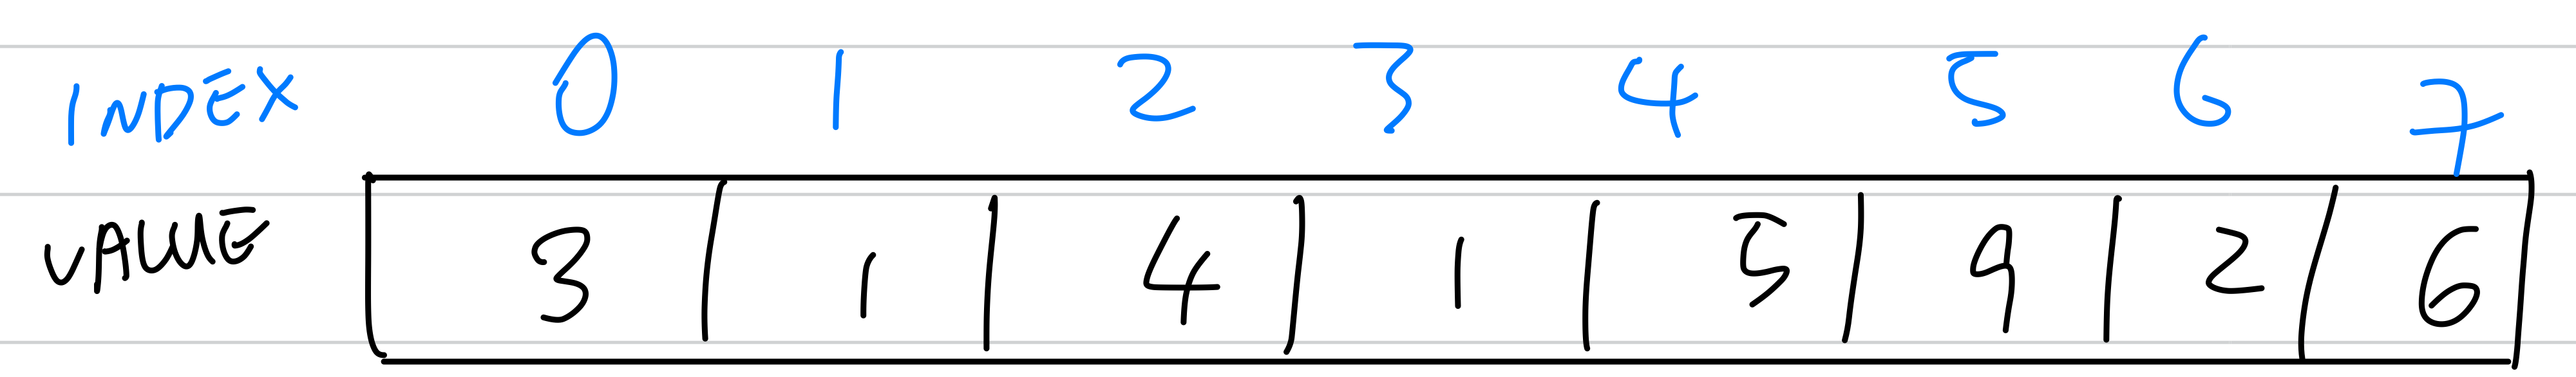
\includegraphics[width=12cm]{images/ch2-arrayindex.png}
\vspace{6mm}

There are two ways of initialising arrays. The first way is to hard-code the elements in the array. The length of the array is inferred by the number of elements given, and it cannot be extended afterwards.

\if\proglang1
\begin{lstlisting}
int[] x = {3,1,4,1,5,9,2,6};
\end{lstlisting}
\else
\begin{lstlisting}
int x[] = {3,1,4,1,5,9,2,6};
\end{lstlisting}
\fi

The second way is when you are not quite sure what the elements of the array are yet, but you must still supply the length of the array.

\if\proglang1
\begin{lstlisting}
int[] x = new int[8];
\end{lstlisting}
\else
\begin{lstlisting}
int x[8];
\end{lstlisting}
\fi

% Translated to Java end

\section{Loops}
\subsection{\texttt{for} loops}
Runs the body a specified number of times.

\begin{lstlisting}
int x[8] = {3,1,4,1,5,9,2,6};
int sum = 0;
for(int i = 0; i < 8; i++) { //loops i=0,1,2,3,4,5,6,7
    sum += x[i];
}
cout << sum << endl; //31
\end{lstlisting}

\begin{lstlisting}
int x[8] = {3,1,4,1,5,9,2,6};
int sum = 0;
for(int i = 7; i >= 0; i--) { //loops i=7,6,5,4,3,2,1,0
    sum += x[i];
}
cout << sum << endl; //31
\end{lstlisting}

\subsection{\texttt{while} loops}
Runs the body until the test is false.
\begin{lstlisting}
int x[8] = {3,1,4,1,5,9,2,6};
int sum = 0;
int i = 0;
while(i<8) { 
    sum += x[i]; //loops i=0,1,2,3,4,5,6,7
    i++;
}
cout << sum << endl; //31
\end{lstlisting}

\begin{lstlisting}
int x[8] = {3,1,4,1,5,9,2,6};
int sum = 0;
int i = 0;
while(i<8&&sum<10) { 
    sum += x[i];
    i++;
}
cout << sum << endl; //14
\end{lstlisting}

\subsection{\texttt{do while} loops}
Runs the body until the test is false. The body will run at least once.

\begin{lstlisting}
bool emergency = false;
do{
    printf("EMERGENCY\n"); //will be printed
}while(emergency);
\end{lstlisting}

\begin{lstlisting}
bool emergency = false;
while(emergency){
    printf("EMERGENCY\n"); //will not be printed
}
\end{lstlisting}

This example yields the same result with while loops because the test is true initially, allowing the loop to run at least once.

\begin{lstlisting}
int x[8] = {3,1,4,1,5,9,2,6};
int sum = 0;
int i = 0;
do { 
    sum += x[i]; //loops i=0,1,2,3,4,5,6,7
    i++;
}while(i<8);
cout << sum << endl; //31
\end{lstlisting}

\subsection{Infinite loops}

If the test case is always true (there is nothing in the loop to make the test false). The loop is an infinite loop\index{infinite loop}, where the loop will not terminate (until resources are used up), and the remaining parts of the program can never be run. In this example, EMERGENCY will be printed forever nonstop.

\begin{lstlisting}
bool emergency = true;
while(emergency){
    printf("EMERGENCY\n");
}
destroy_world(); //will not be run
\end{lstlisting}
\vspace{6mm}

\subsection{\texttt{break}}

\texttt{break} allows you to terminate the loop early.

\begin{lstlisting}
int x[8] = {3,1,4,1,5,9,2,6};
int sum = 0;
int i = 0;
while(i<8) { 
    sum += x[i];
    i++;
    if(sum >= 10) break;
}
cout << sum << endl; //14
\end{lstlisting}

\subsection{\texttt{continue}}

\texttt{continue} allows you to jump to the next iteration, skipping the rest of the current iteration early.

\begin{lstlisting}
int x[8] = {3,1,4,1,5,9,2,6};
int sum = 0;
int i = 8;
while(i>0) {
    i--;
    if(x[i] >= 5) continue;
    sum += x[i];
}
cout << sum << endl; //11
\end{lstlisting}

\subsection{Necessity of \texttt{break} and \texttt{continue}}

% Note that all for loops and do while loops can be written as a while loop.

% \begin{lstlisting}[basicstyle=\rmfamily]
% for(int i = 0; i < <target>; i++) <body> === 
% int i = 0; while(i < <target>) <body> i++;
% \end{lstlisting}

% \begin{lstlisting}[basicstyle=\rmfamily]
% do <body> while(<test>); === <body> while(<test>) <body>
% \end{lstlisting}

Note that the use of \texttt{break} and \texttt{continue} can be avoided by modifying the loop condition and using if statements respectively. 

In fact, plenty of other programming languages do not have \texttt{break} and \texttt{continue}. 

\section{2D arrays}

Don't have time to cover, there should be plenty of resources online on this topic.

\begin{lstlisting}
int x[3][] = {{1,4,7},{2,5,8},{3,6,9}};
cout << x[2][1] << endl; //6
\end{lstlisting}

\subsection{Nested loops}

\begin{lstlisting}
int x[3][] = {{1,4,7},{2,5,8},{3,6,9}};
sum = 0;
for(int i=0;i<3;i++)
    for(int j=0;j<3;j++)
        sum += x[i][j];
cout << sum << endl; //45
\end{lstlisting}

% Translated to Java 
\section{\if\proglang1 Methods \else ~functions \fi}

\if\proglang1 Methods \else ~functions \fi let you organize code better and reduce the amount of repeated code. You can define them by:

\if\proglang1
\begin{lstlisting}[language=,basicstyle=\rmfamily]
public static <return type> <name>(<arguments>){
    return <return value>;
}
\end{lstlisting}
\else
\begin{lstlisting}[language=,basicstyle=\rmfamily]
<return type> function(<arguments>){
    return <return value>;
}
\end{lstlisting}
\fi

For example, this \texttt{fact}\if\proglang1 method \else ~function \fi accepts an integer x, and returns another integer.
\if\proglang1
\begin{lstlisting}
public static int fact(int x){
    int y = 1;
    for(int i = 1; i <= x; i++){
        y *= i;
    }
    return y;
}
//What would happen if we input a negative number?
\end{lstlisting}
\else
\begin{lstlisting}
int fact(int x){
    int y = 1;
    for(int i = 1; i <= x; i++){
        y *= i;
    }
    return y;
}
//What would happen if we input a negative number?
\end{lstlisting}
\fi

This is how you use a\if\proglang1 method \else ~function \fi: 
You could call it by just supplying the argument.

\if\proglang1
\begin{lstlisting}
    System.out.println(fact(6)); //720
\end{lstlisting}
\else
\begin{lstlisting}
    cout << fact(6) << endl; //720
\end{lstlisting}
\fi

Alternatively, we usually would prefer saving the value returned for later use.

\begin{lstlisting}
    int x = fact(6); //720 is now stored in x
\end{lstlisting}

You could use the \texttt{\textbf{void}} keyword to indicate that a\if\proglang1 method \else ~function \fi does not have a return value. For \texttt{void}\if\proglang1 methods \else ~functions \fi, if there is no explicit \texttt{return;} statement, the\if\proglang1 method \else ~function \fi will automatically quit at the end of the\if\proglang1 method \else ~function \fi. 

\if\proglang1
\begin{lstlisting}
import java.util.Scanner;

public static void giveComment(int score){
    if(score >= 70){
        System.out.println("Good job.");
    }else if(score >= 40){
        System.out.println("You got a pass.");
    }else{
        System.out.println("You failed.");
    }
    //automatically quits here
}

public static void main(String args[]){
    Scanner scanner = new Scanner(System.in);  
    int s = scanner.nextInt();
    giveComment(s);
}
\end{lstlisting}
\else
\begin{lstlisting}
void giveComment(int score){
    if(score >= 70){
        printf("Good job.\n");
    }else if(score >= 40){
        printf("You got a pass.\n");
    }else{
        printf("You failed.\n");
    }
    //automatically quits here
}

int main(){
    int s;
    cin >> s;
    giveComment(s);
    //returning 0 is optional for some C/C++ compilers, it is implied it returns 0 normally
}
\end{lstlisting}
\fi

The main\if\proglang1 method \else ~function \fi is just a\if\proglang1 method \else ~function \fi with no arguments and an integer as a return value. The main\if\proglang1 method \else ~function \fi (specially recognized by the compiler) is the point of entry of the program, the program terminates when the main program returns, returning 0 indicates that there is no error, and returning other integers indicate otherwise.
\vspace{6mm}

Note that the giveComment\if\proglang1 method \else ~function \fi must be placed in front of the main\if\proglang1 method \else ~function \fi, or else the main\if\proglang1 method \else ~function \fi could not call the giveComment\if\proglang1 method \else ~function \fi as the\if\proglang1 method \else ~function \fi has not been defined by the time the compiler reads till the main\if\proglang1 method \else ~function \fi. 

% Translated to Java end
\chapter{Data Types}

You have to specify the type of variables when initializing them in C++. Each variable can only be used to store data of a single type.\footnote{Out of scope: this is what we call a strongly typed language} These are also the available types for function arguments and function return values.

\section{Primary data types}
\label{sec:primarydtypes}
\textbf{Primary data types}\index{Primary data types} are those that are not composed of other data types. It is important to distinguish primary data types with other data types (like arrays), as we will see in \cref{sec:passbyref}

Basic knowledge: 1 bit is a single 0 or 1 in memory, 8 bits form 1 byte, we usually discuss memory in terms of bytes instead of bits.

\begin{table}[h]
    \centering
    \begin{tabular}{|m{6em}|m{6em}|m{10em}|m{12em}|}
        \hline
        \textbf{Data Type} & 
        Bytes in Memory & 
        Range & 
        Remarks 
        \\ \hline \hline
        
        \texttt{int} &
        4 & 
        $-2^{31}$ to $2^{31}-1$ (i.e. -2147483648 to 2147483647) &
        
        \\ \hline
        
        \texttt{bool} &
        1 & 
        \texttt{true} / \texttt{false}  &
        \tablefootnote{Out of scope: in C++ bool is a primary data type, in C you will have to include stdbool.h to use it.} 
        \\ \hline
        
        \texttt{char} &
        1 & 
        /  &
        Stored using an integer, the ASCII code of the character
        \\ \hline
        
        \texttt{float} &
        4 &
        A large range \textcolor{gray}{ (~$-10^{38}$ to $10^{38}$)} &
        Stores numbers with decimal places
        \\ \hline
        
        \texttt{double} &
        8 & 
        A large range \textcolor{gray}{ (~$-10^{308}$ to $10^{308}$)} &
        Stores numbers with decimal places
        \\ \hline
    \end{tabular}
\end{table}

\pagebreak

These are variants of integers. They are of less importance.\footnote{Reference: \href{https://en.cppreference.com/w/cpp/language/types}{https://en.cppreference.com/w/cpp/language/types}, the range and bytes occupied differs for different version of C++}

\begin{table}[h]
    \centering
    \begin{tabular}{|m{6em}|m{6em}|m{10em}|m{12em}|}
        \hline
        \textbf{Data Type} & 
        Bytes in Memory & 
        Range & 
        Remarks 
        \\ \hline \hline
        
        \texttt{unsigned} &
        4 & 
        $0$ to $2^{32}-1$ (i.e. 0 to 4294967295) &
        Cannot store negative numbers, yet approximately double the range.
        \\ \hline
        
        \texttt{short} &
        2 & 
        $-2^{15}$ to $2^{15}-1$ (i.e. -32768 to 32767) &
        Half the size of an \texttt{int}
        \\ \hline
        
        \texttt{long long} &
        8 & 
        $-2^{63}$ to $2^{63}-1$ &
        Double the size of an \texttt{int}
        \\ \hline
        
    \end{tabular}
\end{table}

\section{Integer overflow\index{overflow}}

As you saw in the last section, integers have a limited range. Overflow occurs when the value we want to store is out of the range that the data type can represent. 

For integers (\texttt{int}, \texttt{unsigned}, \texttt{short}, \texttt{long long}), the value it represents will go to the other end of the range when they overflow.\footnote{Reason behind out of scope: requires understanding of two's compliment}. 

For example,
\begin{lstlisting}
int x = 2147483647;
cout << "Before overflow: " << x << endl; //2147483647
x += 1;
cout << "After overflow: " << x << endl; //-2147483648

unsigned y = 4294967295;
cout << "Before overflow: " << y << endl; //4294967295
y += 1;
cout << "After overflow: " << y << endl; //0
\end{lstlisting}

\section{Floating point values}

OK, the range of floating point values\index{floating point values} (\texttt{float} and \texttt{double}) are much larger than ints, so is it a good idea to use them all the time? NO!

Floating point values store values inaccurately, and \textbf{rounding errors} accumulate. Even though using \texttt{double} reduces the rounding error, floating point values are still nasty in some ways. 

You are advised to only use \texttt{double} to store numbers with decimal points and very large numbers (those can't be represented by \texttt{long long}). And never use \texttt{float}\footnote{Memory usage is not a problem nowadays}.

\section{Boolean operators}

A Boolean\index{Boolean} variable (\texttt{bool}) can be either \texttt{true} or \texttt{false}. There are three operations that we can perform on \texttt{bool}s. Including AND (\&\&), OR (\textbar\textbar), NOT (!).

\begin{table}[h]
    \centering
    \begin{tabular}{|m{4em}|m{4em}|m{4em}|m{4em}|m{4em}|}
        \hline
        a & 
        b & 
        a \&\& b & 
        a\textbar\textbar b & 
        !a 
        \\ \hline \hline
        
        true & 
        true & 
        true & 
        true & 
        false 
        \\ \hline
        
        true & 
        false & 
        false & 
        true & 
        false 
        \\ \hline
        
        false & 
        true & 
        false & 
        true & 
        true 
        \\ \hline
        
        false & 
        false & 
        false & 
        false & 
        true 
        \\ \hline
        
    \end{tabular}
\end{table}

C/C++ recognizes 0 as false and other non-zero values as true. It is common to use 1 instead of true\footnote{a convention} and 0 instead of false.

You could do \texttt{while(true) ...} for an infinite loop, but you might as well do \texttt{while(1) ...}
\vspace{6mm}

Order of precedence: ! $>$ \&\& $>$ \textbar\textbar

For example, 

!0 \textbar\textbar 0 \&\& 1

= (!0) \textbar\textbar 0 \&\& 1

= 1 \textbar\textbar 0 \&\& 1

= 1 \textbar\textbar (0 \&\& 1)

= 1 \textbar\textbar 0

= 1

\subsection{Bitwise operators}

\textit{Difficult topic}
\vspace{6mm}

Don't have time to cover, there should be plenty of resources online on this topic. 

Yet, it is important for senior group contestants as this kind of questions seem common. 

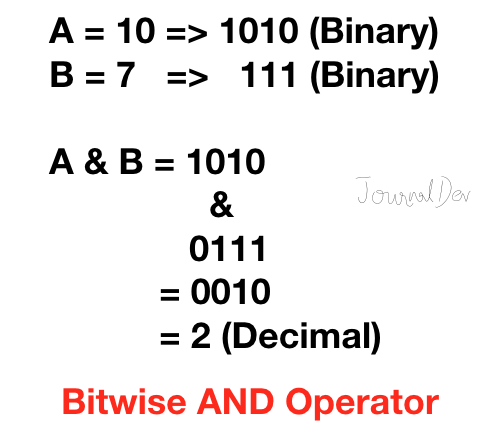
\includegraphics[width=7cm]{ch3-bitwise.png}
\footnote{Reference: \href{https://www.digitalocean.com/community/tutorials/python-bitwise-operators}{https://www.digitalocean.com/community/tutorials/python-bitwise-operators}}

\section{Characters are integers}

Let's run some C++ code.

\begin{lstlisting}
char a = 'a'; //we use single quotes for characters and double quotes for strings
printf("%d %c\n",a,a); //97 a
a = 97;
printf("%d %c\n",a,a); //97 a
a = 65;
printf("%d %c\n",a,a); //65 A
a += 1;
printf("%d %c\n",a,a); //66 B
\end{lstlisting}

It seems that each character is associated with an integer. That's right! 128 (later extended to 256) frequently used characters are chosen (including the English letters, digits, and common symbols) and they are associated with an integer between 0 and 127.\footnote{ASCII Table: \href{https://simple.wikipedia.org/wiki/ASCII}{https://simple.wikipedia.org/wiki/ASCII}}

We can perform arithmetic operations with \texttt{char} variables, as they are just integers! 

\section{Type casting}

We can covert values from one type to another, by putting the target type, enclosed with parenthesis, on the left of the value.

\begin{lstlisting}
cout << (int) 40.9 << endl; //40
cout << (bool) -1 << endl; //1
cout << (int) 'a' << endl; //97
\end{lstlisting}

When floating point values are cast to an integer, it is \textbf{rounded down}. Non-zero values are cast to \texttt{true}, hence \texttt{1} is displayed. The character \texttt{a} is converted to an integer based on its ASCII code.

Type cast is done automatically whenever possible\footnote{When it is not possible, e.g. from integer array to character, an error would occur} when a value is assigned to a variable of a different type. Note that type of a variable cannot be changed. 

\begin{lstlisting}
int x;
x = 40.9; //x is an int, so 40.9 got cast into an integer, 40, before storing into x
cout << x << endl; //40
\end{lstlisting}

\section{Strings}

\textit{Of less importance, except operation on string variables}
\vspace{6mm}

Strings are best understood as an array of characters, we would store them using a character array such as  \texttt{char s[10] = "Hello";} \footnote{We would avoid using the type \texttt{string} in C++, but use character arrays to store strings}, but there are a few nasty catches.

\subsection*{Strings terminate with a null character \texttt{\textbackslash 0}}

Hm, the word \texttt{hello} only has 5 characters, can we do \texttt{char s[5] = "Hello";} instead? Not really.

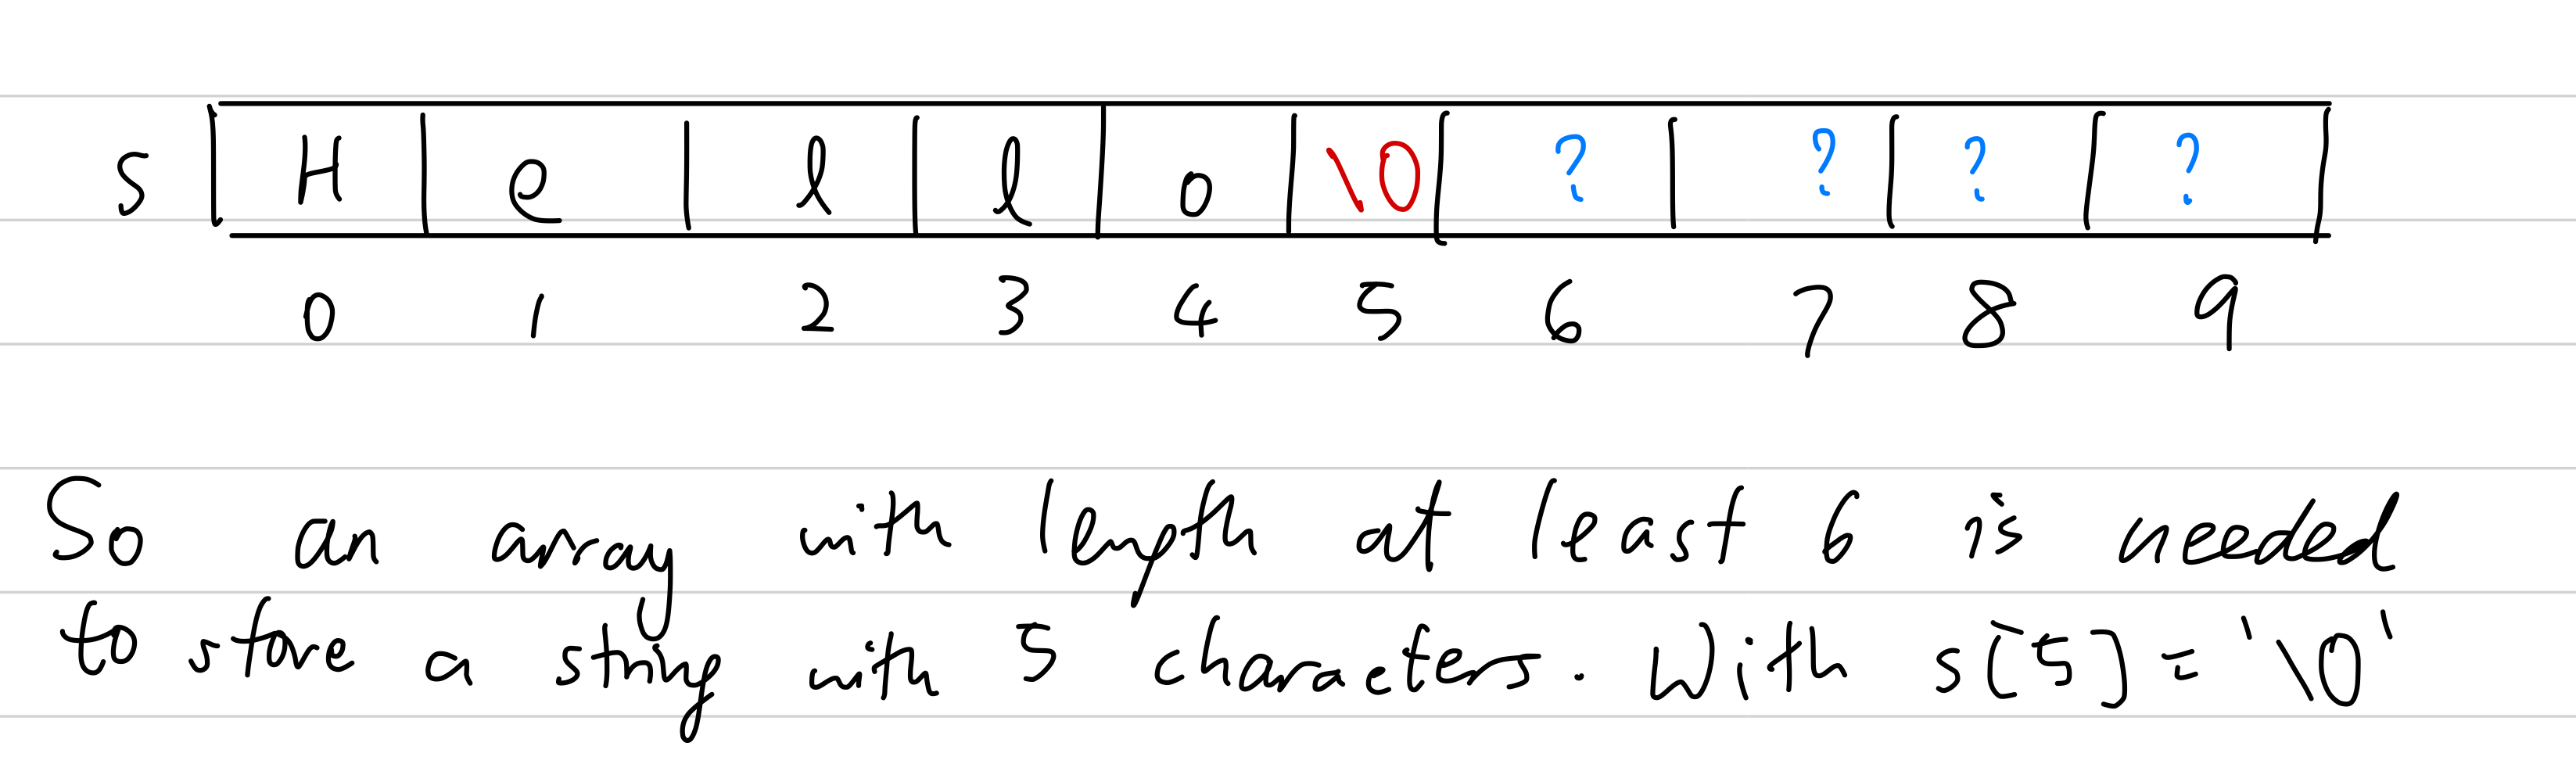
\includegraphics[width=15cm]{ch3-nullstring.png}

The \texttt{\textbackslash 0} (ASCII code = 0) indicates the end of a string, it is necessary for C/C++ programs so that they could identify when the string ends. If you remove it something bad would happen...

Don't trust me? Try running:

\begin{lstlisting}
char s[4] = "FGH";
s[3] = 'I'; //Remove the \0 character and replace it by character I
cout << s << endl; //FGHI followed by a bunch of nonsense, the nonsense is different everytime we run the program

char s1[7] = { 'A', 'B', 'C', '\0', 'D', 'E', '\0'};
cout << s1 << endl; //ABC
\end{lstlisting}

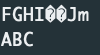
\includegraphics[width=3cm]{ch3-beyondnull.png}

The first example shows what happens when we explicitly remove the null character at the end of the string. (By replacing \texttt{FGH\textbackslash 0} with \text{FGHI}) It attempts to access and print things beyond the memory allocated. (see chapter 5 for more details)

The second example verifies that the null character is recognized by C/C++ as the end of the string, despite having some other contents after the null character.

\textbf{So we always have to reserve one more space for the null character.}

\subsection*{\texttt{cin} obtains input word by word}

This example shows that \texttt{cin} only catches the first word and store it in \texttt{s2}, while leaving other words for future calls of \texttt{cin}.

\begin{lstlisting}
char s2[20], s3[20];
cin >> s2; //You inputted Hello world
cout << s2 << endl; //Hello

cin >> s3; //The computer did not ask for your input
cout << s3 << endl; //world
\end{lstlisting}

\label{sec:cingetline}
However, sometimes you want to obtain a whole line of text input rather than just a word. You could use \texttt{cin.getline}. It accepts two arguments, first the string variable (the character array you defined), second the maximum amount of characters it should get (you have to set it less than or equal to the size of the chracter array)

\begin{lstlisting}
char s4[20];
cin.getline(s4,20); //You inputted Good morning
cout << s4 << endl; //Good morning
\end{lstlisting}

Unfortunately it is not as simple as that, things get complicated when you have other \texttt{cin}s in the same program.

\begin{lstlisting}
char s2[20], s3[20];
cin >> s2; //You inputted Hello world
cout << s2 << endl; //Hello

cin >> s3; //The computer did not ask for your input
cout << s3 << endl; //world

char s4[20];
cin.getline(s4,20); //The computer did not ask for your input
cout << s4 << endl; //Probably a next line symbol (\n)
\end{lstlisting}

This behaviour is probably\footnote{Who is certain about this chaos?} due to the next line symbol of the Hello world line has not been read (\texttt{\textbackslash n} is inputted when you press enter to confirm your input), and \texttt{cin.getline} reads the text until it hits a next line symbol, and that is the only thing stored in \texttt{s4}.

What you could do is use \texttt{cin.clear()} and \texttt{cin.ignore(10000,'\textbackslash n')} (both are required) before \texttt{cin.getline}, in order to clear the buffer.

\begin{lstlisting}
char s2[20], s3[20];
cin >> s2; //You inputted Hello world
cout << s2 << endl; //Hello

cin >> s3; //The computer did not ask for your input
cout << s3 << endl; //world

char s4[20];
cin.clear();
cin.ignore(10000, '\n');
cin.getline(s4,20); //You inputted Good morning
cout << s4 << endl; //Good morning
\end{lstlisting}

Alternatively, you could call \texttt{cin.getline} twice, the first one to read the previous line, and the second one to actually read your input. The result of the first read is overwritten by the second one as desired.

\begin{lstlisting}
char s2[20], s3[20];
cin >> s2; //You inputted Hello world
cout << s2 << endl; //Hello

cin >> s3; //The computer did not ask for your input
cout << s3 << endl; //world

char s4[20];
cin.getline(s4,20); //read the previous line
cin.getline(s4,20); //You inputted Good morning
cout << s4 << endl; //Good morning
\end{lstlisting}

\subsection{Strings VS string variables}

The following two restrictions concern string variables but not strings. Now let's differentiate strings and string variables.
\vspace{6mm}

Strings are hard coded in the source code, only for one time use. Normal users (not you, you are the programmer) cannot change it.

String variables are character arrays that are used to store strings. They can be changed by users if their values are obtained by input, e.g. \texttt{cin}. 

\subsection*{String variables cannot be compared normally}

You can compare them normally using comparison operators.

\begin{lstlisting}
cout << ("ABC"=="DEF") << endl; //0
cout << ("ABC" < "DEF") << endl; //1 (why?)
cout << ("abc" <= "ABC") << endl; //0 (why?)
\end{lstlisting}

Sadly they return unmeaningful results when string variables are being compared. (use strcmp instead)\footnote{Reason out of scope: because the references of the arrays are compared instead of their values. You may understand more in Chapter 5 but the full concept is not necessary}

\begin{lstlisting}
char s5[20] = "ABC", s6[20] = "ABC", s7[20] = "DEF";
cout << (s5==s5) << endl; //1
cout << (s5==s6) << endl; //0
cout << (s5<s6) << endl; //0
\end{lstlisting}

Use \texttt{strcmp} instead (will be formally introduced next section)
\begin{lstlisting}
char s8[20] = "ABC", s9[20] = "ABC", s10[20] = "DEF";
cout << strcmp(s8,s9) << endl; //0, implying s8 equals s9
cout << strcmp(s8,s10) << endl; //negative value, implying s8 < s10
\end{lstlisting}

\subsection*{The whole string variable cannot be reassigned}

Thought you could do this? Nah...

\begin{lstlisting}
char s11[20] = "ABCD";
s11 = "XYZ"; //SYNTAX ERROR
\end{lstlisting}

Well you could do the following instead if you are desperate, but it is much better using \texttt{strcpy} (will be formally introduced next section)

\begin{lstlisting}
//desperate way:
s11[0] = 'X'; 
s11[1] = 'Y'; 
s11[2] = 'Z'; 
s11[3] = '\0'; 

//better way:
strcpy(s11,"PQR");
\end{lstlisting}


\subsection{Operation on string variables (IMPORTANT)}

\begin{lstlisting}
#include <cstring>
\end{lstlisting}

\begin{table}[h]
    \centering
    \begin{tabular}{|m{9em}|m{25em}|}
        \hline
        \textbf{Function} & 
        Usage 
        \\ \hline \hline
        
        \texttt{strlen(s)} &
        Get string length
        \\ \hline
        
        \texttt{strcpy(s1, s2)} &
        Copy value stored in \texttt{s2} to \texttt{s1} 
        \\ \hline
        
        \texttt{strcat(s1, s2)} &
        Concatenate (i.e. combine) the two strings, store it in \texttt{s1} 
        \\ \hline
        
        \texttt{strcmp(s1, s2)} &
        Compare two strings, returns 0 if \texttt{s1} = \texttt{s2}, returns a negative number if \texttt{s1} $<$ \texttt{s2}, returns a positive number if \texttt{s1} $>$ \texttt{s2}. (In dictionary order with respect to ASCII code)
        \\ \hline
    \end{tabular}
\end{table}

You are advised to try out these operations yourself, I am sure you will find surprises.

\section{Conclusion and further resources}

\href{https://www.youtube.com/watch?v=Zy2bNkSxv8M}{This video}\footnote{Link: \href{https://www.youtube.com/watch?v=Zy2bNkSxv8M}{https://www.youtube.com/watch?v=Zy2bNkSxv8M}} summarizes some more nasty things about strings. Bear in mind what you can and what you can't do with them.
\vspace{6mm}

\begin{center}
\textit{The most comfortable type to deal with are integers.}
\end{center}

\chapter{Recursion}

\textit{Difficult topic}
\vspace{6mm}

Recursive functions are those which call themselves again inside their function body, for example, the \texttt{fact} function that I will introduce down the chapter.

It might be difficult to get right and understand at first for learners, but it simplifies code once you get used to it. The best way to master it is through looking at more examples. You can see more examples on recursion in the mycodeschool playlist.

\section{Further resources (Ch 4-6)}

Playlists by 
\href{https://www.youtube.com/user/mycodeschool}{mycodeschool}\footnote{Link: \href{https://www.youtube.com/user/mycodeschool}{https://www.youtube.com/user/mycodeschool}}
that focus on 
\href{https://www.youtube.com/playlist?list=PL2\_aWCzGMAwLz3g66WrxFGSXvSsvyfzCO}{recursion}\footnote{Link: \href{https://www.youtube.com/playlist?list=PL2\_aWCzGMAwLz3g66WrxFGSXvSsvyfzCO}{https://www.youtube.com/playlist?list=PL2\_aWCzGMAwLz3g66WrxFGSXvSsvyfzCO}}, 
\href{https://youtube.com/playlist?list=PL2_aWCzGMAwLZp6LMUKI3cc7pgGsasm2_}{pointers}\footnote{Link: \href{https://youtube.com/playlist?list=PL2_aWCzGMAwLZp6LMUKI3cc7pgGsasm2_}{https://youtube.com/playlist?list=PL2\_aWCzGMAwLZp6LMUKI3cc7pgGsasm2\_}} and 
\href{https://www.youtube.com/playlist?list=PL2_aWCzGMAwI3W_JlcBbtYTwiQSsOTa6P}{data structures (linked lists, stacks, queues)}\footnote{Link: \href{https://www.youtube.com/playlist?list=PL2_aWCzGMAwI3W_JlcBbtYTwiQSsOTa6P}{https://www.youtube.com/playlist?list=PL2\_aWCzGMAwI3W\_JlcBbtYTwiQSsOTa6P}}.
mycodeschool explains concepts about computing pretty well. You can also watch his other playlists if interested.

\section{Example: Factorial function}

In \cref{sec:functions}, we wrote a non-recursive function that calculates the factorial of a number.
\begin{lstlisting}
int fact(int x){
    int y = 1;
    for(int i = 1; i <= x; i++){
        y *= i;
    }
    return y;
}
\end{lstlisting}

Here is an equivalent function that is recursive.

\begin{lstlisting}
int fact(int x){
    if(x==0) return 1; //0! = 1
    else return x*fact(x-1); //x! = x*(x-1)!
}
\end{lstlisting}

Let's analyse the recursive version of the function. Because it is simple\footnote{Out of scope: I call a function "simple" in this chapter if it does not invoke any side effects, such as printing something on the screen or accessing (read or write) the value of global variables. The definition is intentionally hidden for easier understanding.} we can use an equational method to analyse the function. For example, we can analyse the return value of \texttt{fact(4)} as follows:

\textit{To think about: What happens if we enter a negative number to both functions?}

\section{Example: Exponentiation}

Here is a recursive function to calculate $x^n$. \textit{Exercise: Implement a non-recursive version of the function.}

\begin{lstlisting}
int exp(int x, int n){
    if(n == 0) return 0; //x^0 = 1
    else return x*exp(x,n-1); //x^n = x*x^(n-1)
}
\end{lstlisting}

The analysis is similar to the factorial function. Here is an example of examining what \texttt{exp(2,5)} will return.

\begin{lstlisting}
exp(2,5)
= 2*exp(2,4)            (by the else clause of exp)
= 2*2*exp(2,3)          (by the else clause of exp)
= 2*2*2*exp(2,2)        (by the else clause of exp)
= 2*2*2*2*exp(2,1)      (by the else clause of exp)
= 2*2*2*2*2*exp(2,0)    (by the else clause of exp)
= 2*2*2*2*2*1           (by the if clause of exp)
= 32                    (just arithmetic)
\end{lstlisting}

\section{Example: Fast Exponentiation}

The above method of calculating $x^n$ works but it is inefficient (linear in $n$, i.e. $O(n)$, see \cref{sec:bigO}). 

People figured out a more efficient way of calculating $x^n$ (logarithmic in $n$, i.e. $O(\log n)$, see \cref{sec:bigO}). 

The mathematical formula is as follows:

\[
    x^n = \begin{cases}
    x, & \text{for } n = 1 \\
    (x^2)^{\frac{n}{2}}, & \text{for even } n \\
    x \times x^{n-1} & \text{for odd } n \neq 1\\
    \end{cases}
\]

% \begin{center}
% $x^1 = x$

% $x^{2n} = (x^2)^n$

% $x^{2n+1} = x \times (x^2)^n$
% \end{center}

For example, $2^{10} = 4^5 = 4\times 16^2 = 4\times 256 = 1024$.

The recursive code is as follows: \textit{Exercise: Implement a non-recursive version of the function.}

\begin{lstlisting}
int fastExp(int x, int n){
    if(n == 1) return x; //x^1 = x
    else if(n%2==0) return fastExp(x*x, n/2); 
        //x^n = (x*x)^(n/2) for even n
    else return x*fastExp(x*x,n/2); 
        //x^n = x*(x*x)^((n-1)/2) for odd n (n/2 is automatically rounded down in C++)
}
\end{lstlisting}

\section{Call stack}

Not every recursive function can be analysed in this way.\footnote{Out of scope: Because some functions are not "simple", that is, they invoke side effects.} To know more about recursive functions we need to learn about how functions are treated in computer memory. Internally, there is a \textbf{call stack}\index{call stack} that stores information about each function call (e.g. the values of the variables, what is left to do) so that they could resume in order.

The figure shows what happens when I call \texttt{fact(4)}.

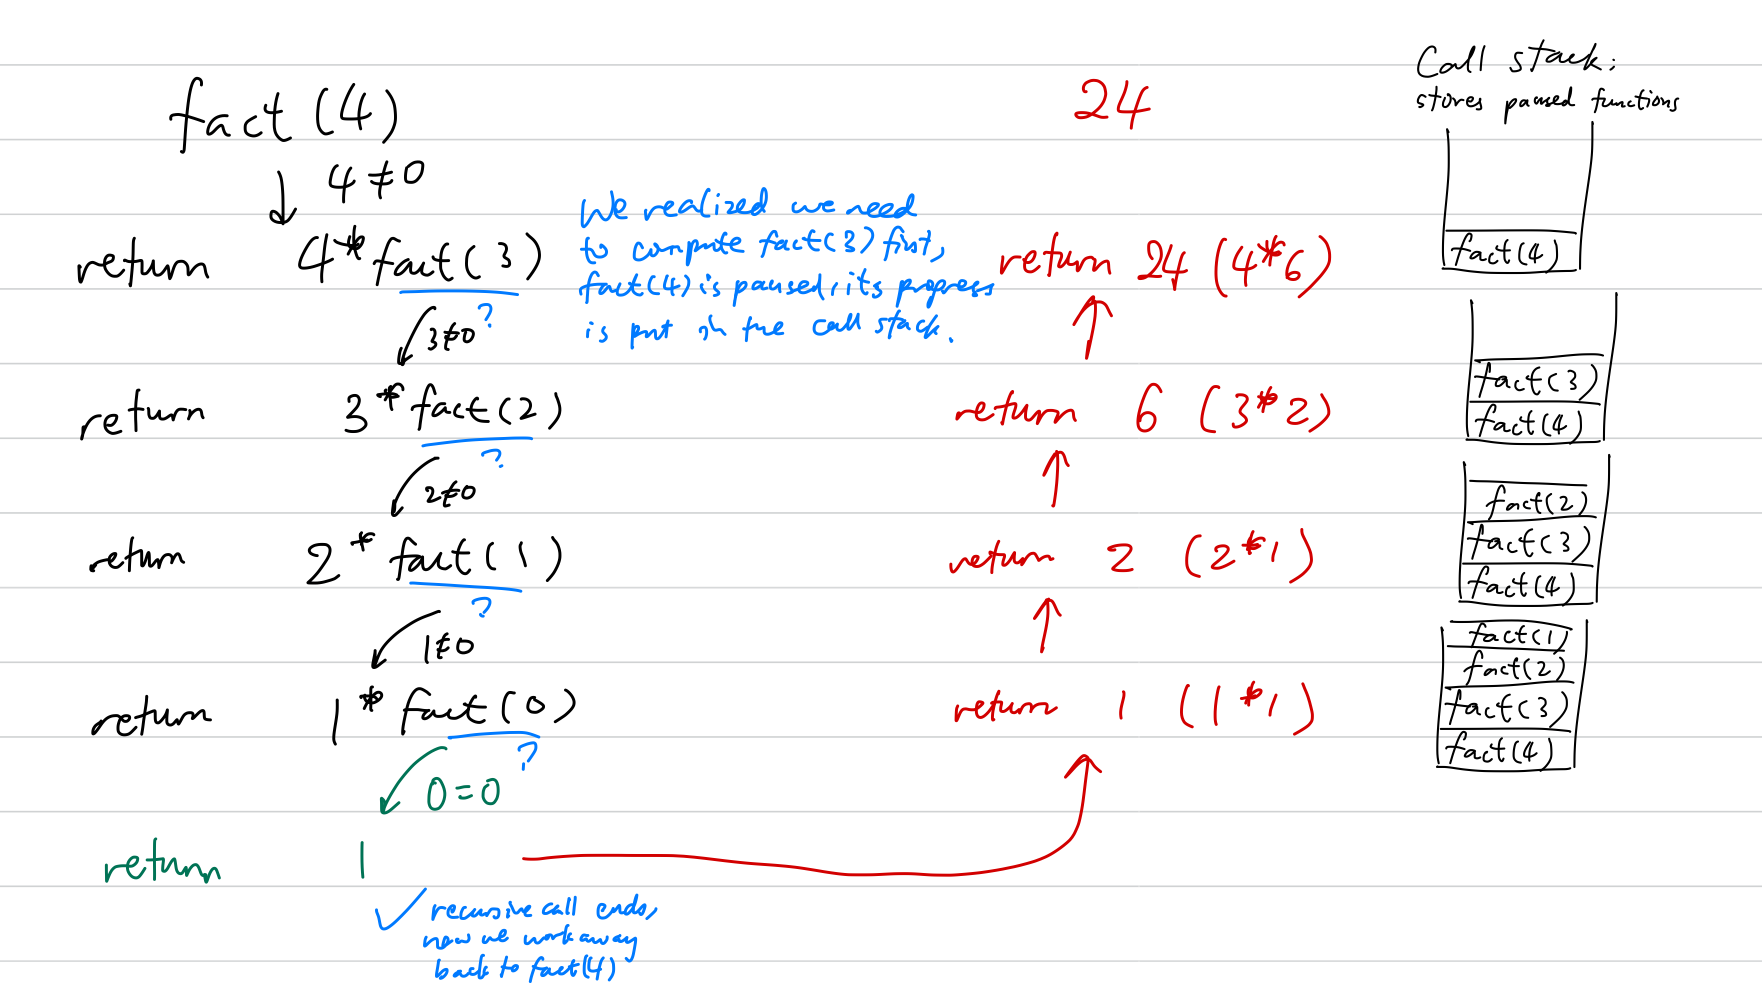
\includegraphics[width=15cm]{ch4-factorial.png}

\texttt{fact(4)} is called, realizing it needs \texttt{fact(3)} to finish, the program pauses \texttt{fact(4)}, and puts it in the call stack, so that it remembers to resume it after getting the result of \texttt{fact(3)}. A similar process happened for \texttt{fact(3)}, \texttt{fact(2)} and \texttt{fact(1)}. Finally, when \texttt{fact(0)} is called, there is no need to rely on other function calls to obtain the return value 1. We call \texttt{fact(0)} the \textbf{base case}\index{base case}. With the result of \texttt{fact(0)}, \texttt{fact(1)} can be resumed, \texttt{fact(1)} is removed from the call stack and its result is computed. A similar process happened for \texttt{fact(2)}, \texttt{fact(3)} and \texttt{fact(4)}, giving the required result finally.
\vspace{6mm}

\section{Example: Weird function}

We would use the call stack method to analyse the output of \texttt{f(0)}\footnote{Modified from HKOI 2022 Heat Senior Group \url{https://assets.hkoi.org/ref/2022hs.pdf}} . You can see the equational method does not work\footnote{Out of scope: because it involves accessing (reading and writing) the array \texttt{a}, this counts as a side effect.}.

\begin{lstlisting}
int a[7] = {3, 6, 8, 2, 5, 1, 2};
int f(int x) {
    if (x >= 3)
        return a[x];
    else {
        a[x] += f(x + 1);
        a[x] += f(x + 2);
        return a[x];
    }
}
int main() {
    cout << f(0);
    return 0;
} 
\end{lstlisting}

This kind of non-simple functions occur frequently in programming competitions but they are of less importance in university.\footnote{Recursive functions with side effects are less mathematically pleasing.}

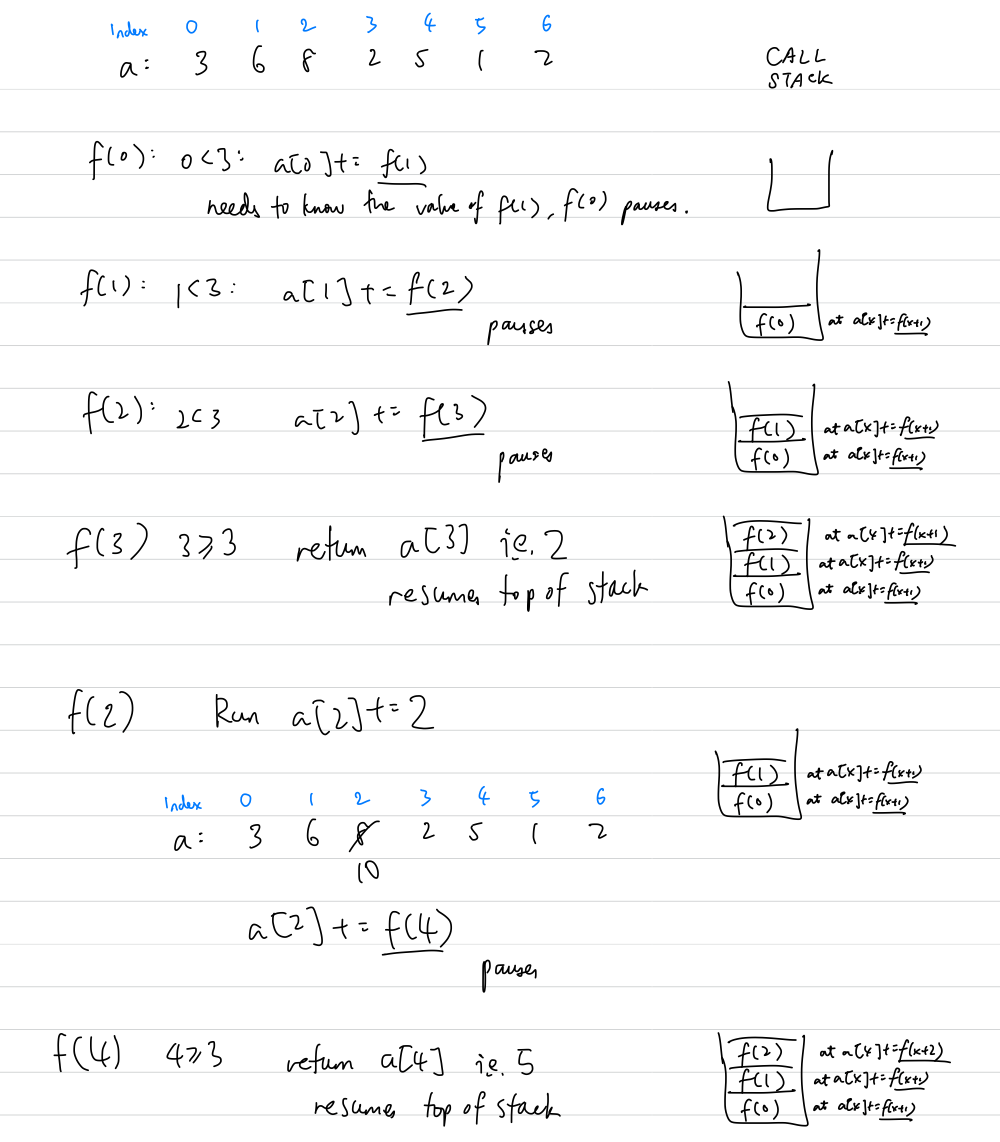
\includegraphics[width=15cm]{images/ch4-rec1.png}

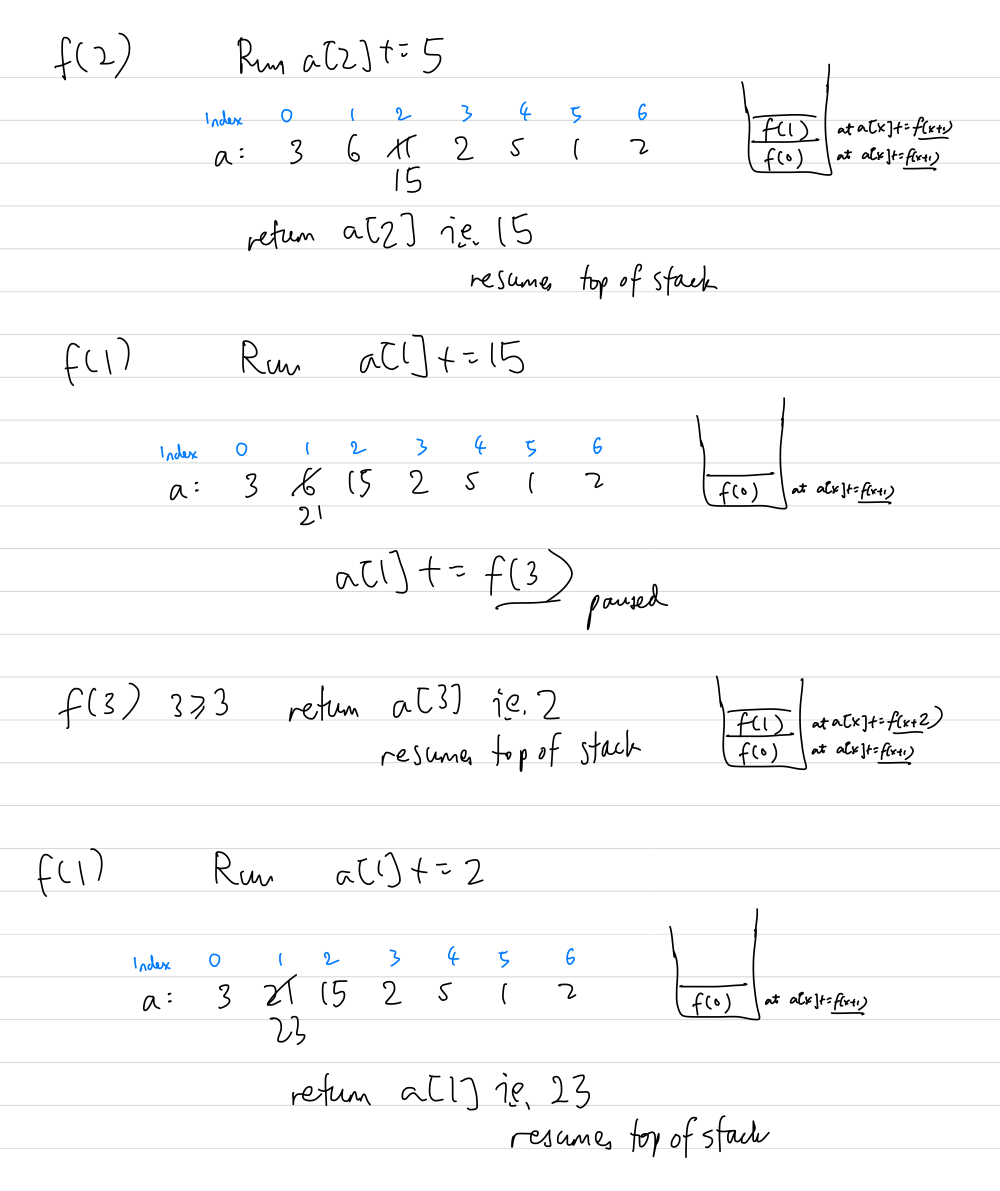
\includegraphics[width=15cm]{images/ch4-rec2.png}

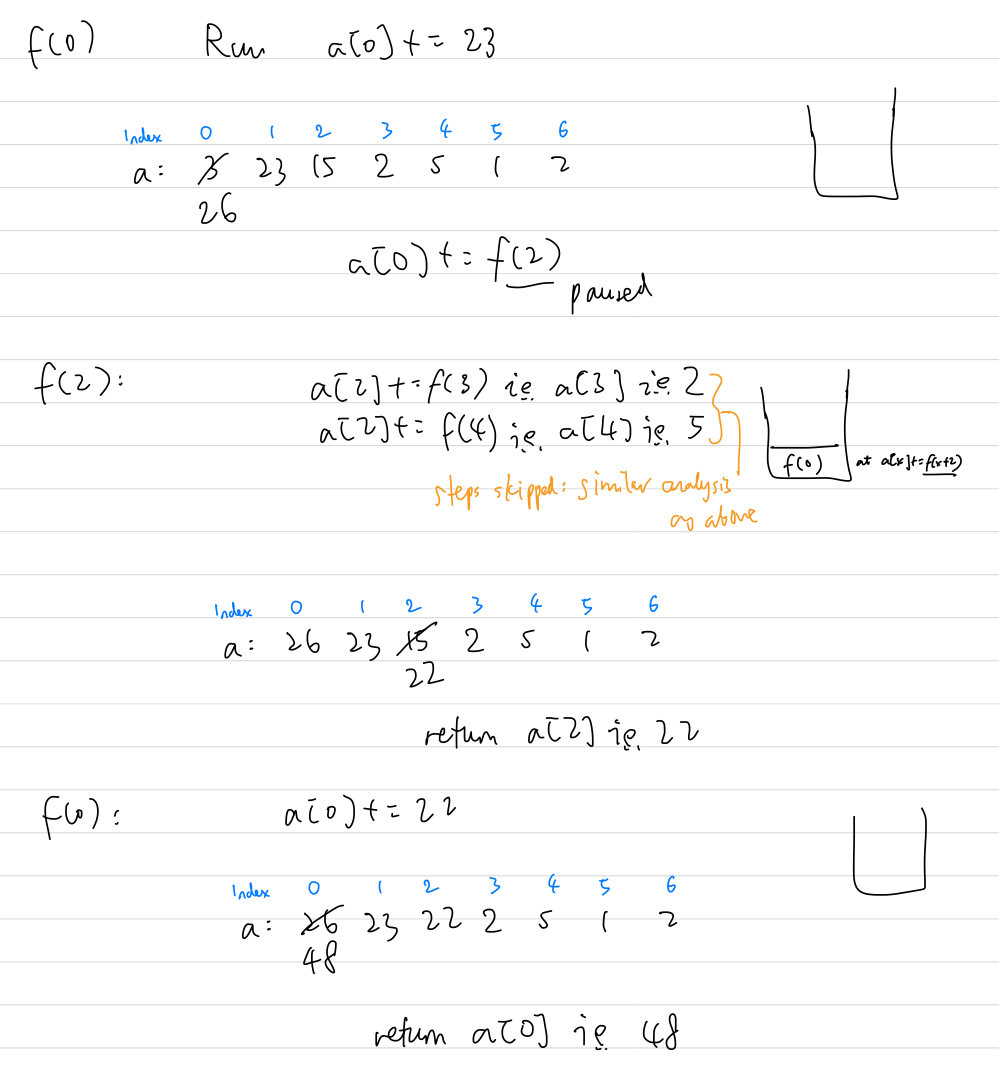
\includegraphics[width=15cm]{images/ch4-rec3.png}
\chapter{Arrays and Linked Lists}
% Translated into Java (whole chapter)

\label{sec:arraychap}
We will talk more about arrays and new concepts including linked lists, pointers and time complexity in this chapter.

\section{Arrays in memory}

Let's go back to the example in \cref{sec:arrayintro}.

\if\proglang1
\begin{lstlisting}
int[] x = {3,1,4,1,5,9,2,6};

System.out.println(x[0]); //3 
System.out.println(x[4]); //5
System.out.println(x[7]); //6 (last element)
System.out.println(x[8]); //Error 
\end{lstlisting}
\else
\begin{lstlisting}
int x[8] = {3,1,4,1,5,9,2,6};
//alternatively: int x[] = {3,1,4,1,5,9,2,6}; length of array can be omitted as the compiler can derive it from the right hand side

cout << x[0] << endl; //3 
cout << x[4] << endl; //5
cout << x[7] << endl; //6 (last element)
cout << x[8] << endl; //unexpected value (Why?)
\end{lstlisting}
\fi

\if\proglang1 To understand more about arrays, \else The reason for \texttt{x[8]} to return an unexpected value rather than an error is pretty interesting. To understand that, \fi you will need to know how arrays are stored in memory, and how array elements are accessed. 

A \textbf{continuous} memory is allocated for each array. As indicated in the figure.

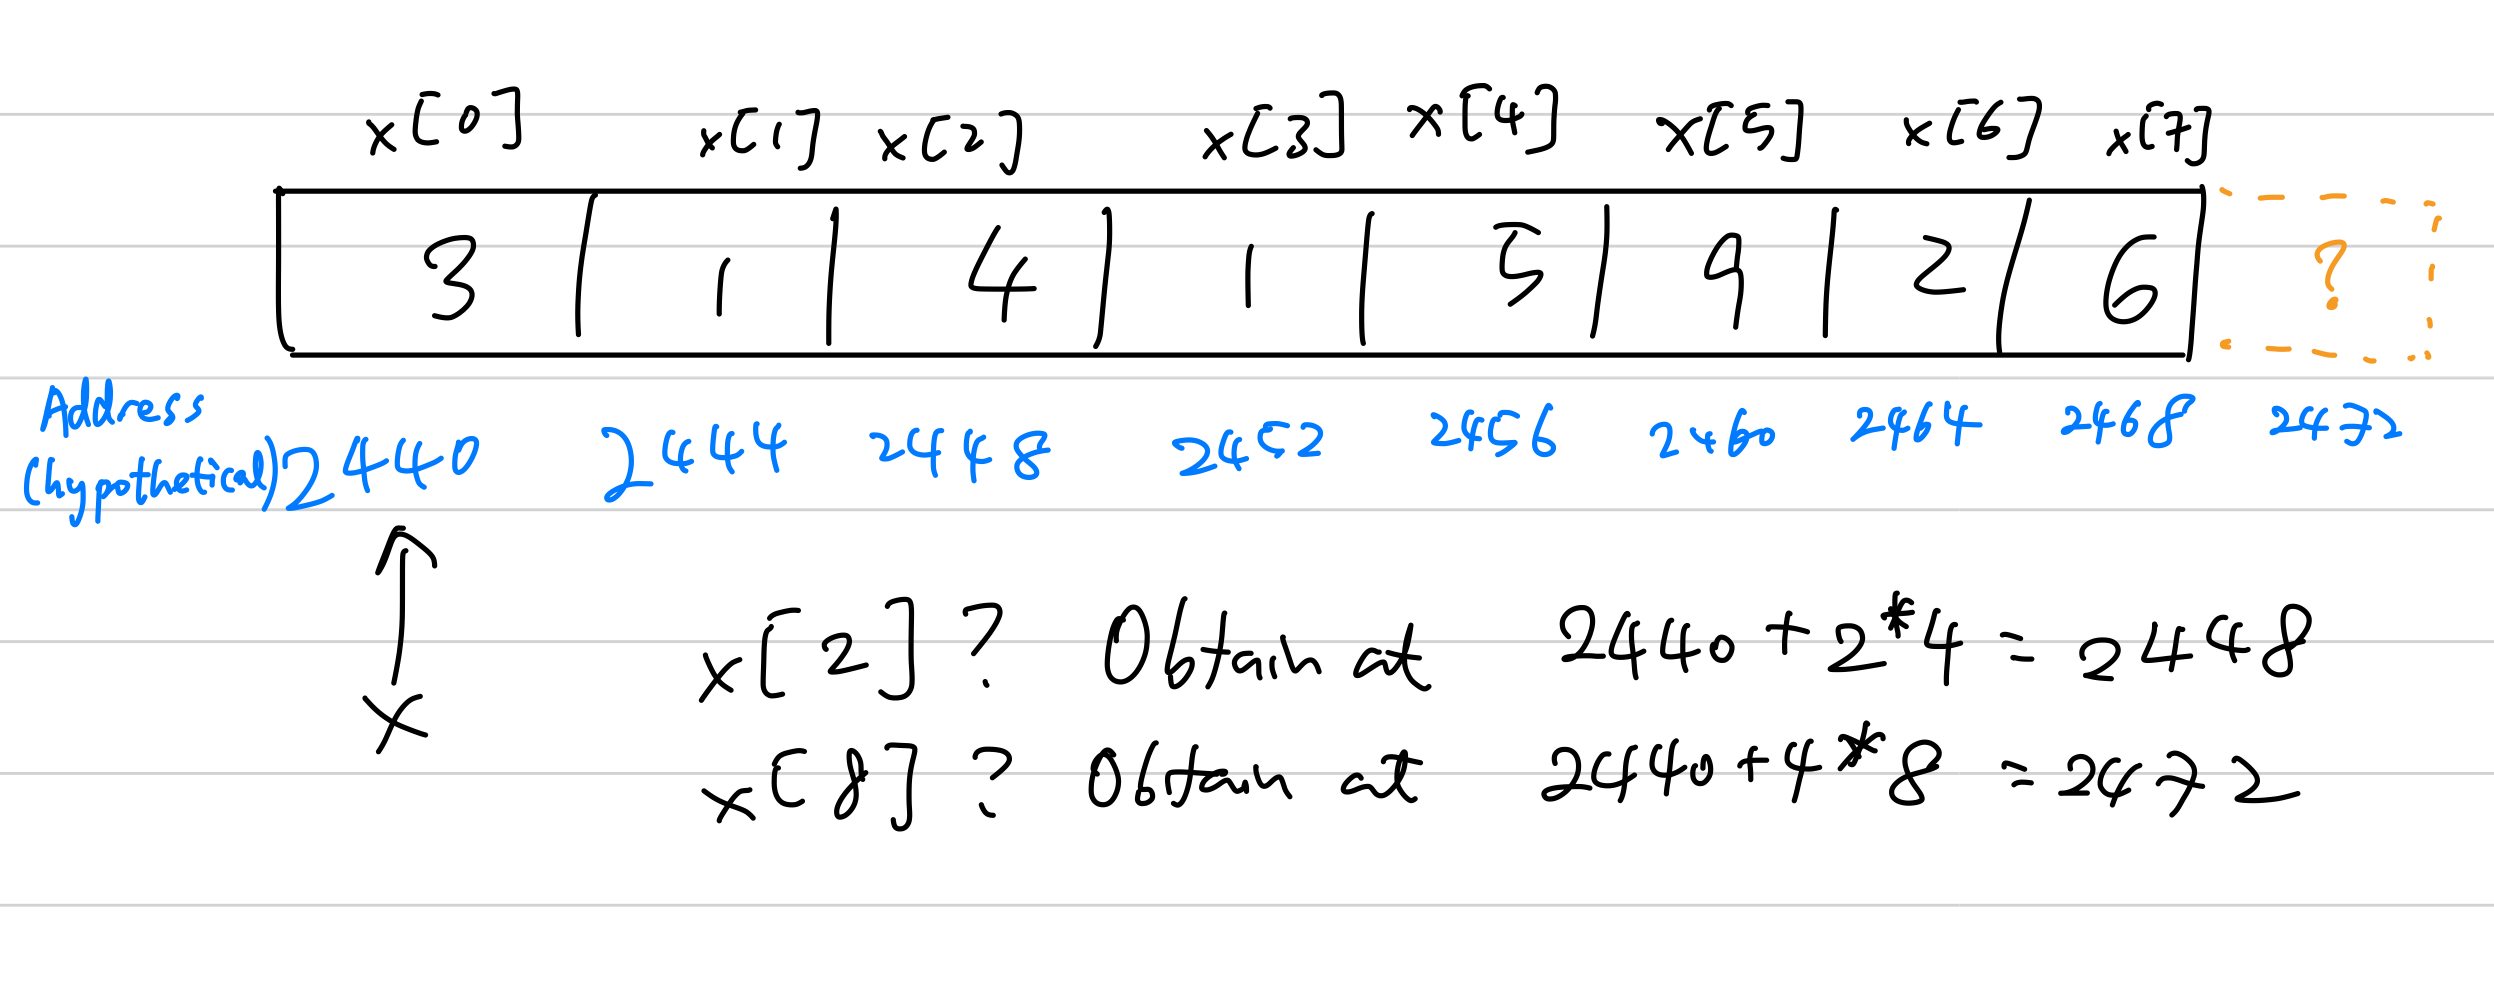
\includegraphics[width=13cm]{ch5-array.png}

\if\proglang1 Java \else ~C++ \fi stores the \textbf{base address}\index{base address} of the array x, say at location 2440. Then to obtain \texttt{x[k]}, it will calculate the address that it needs to retrieve by $2440 + k*4$, the $*4$ is there because each integer occupies 4 bytes of memory, the multiplier is different depending on different data types. 

For example, when querying \texttt{x[4]}, we obtained it from address $2440+16 = 2456$. 

So, when querying \texttt{x[8]}, we obtained it from address $2440+32 = 2472$. What is in address 2472? We don't know! It is just a bunch of random 0s and 1s last modified by other programs. 


\if\proglang1 The \else If you run this program multiple times, the result printed is different, this is because the \fi base address allocated for the array by the program is different every time. 

As the location of \texttt{x[8]} is different, it probably stores a different sequence of 0s and 1s. While x[0..7] are the same, because that is what \texttt{int x[8] = \{3,1,4,1,5,9,2,6\};} does, put 3 at base address, put 1 at base address + 4, put 4 at base address + 8 ..., once the base address is allocated.

\section{Pointers}

\textit{Of less importance, difficult topic}


Don't have time to cover, there should be plenty of resources online on this topic, including mycodeschool's playlist on pointers.

\section{Pointers and arrays}
\label{sec:passbyref}
\textit{Difficult topic}


Although we did not cover pointers in depth, it is important to understand the usage of pointers in manipulating arrays. 

First, we need to understand that there are two ways values are passed by a function call, that is, \textbf{call by reference}\index{call by reference} and \textbf{call by value}\index{call by value}, you will need to be able to distinguish when each type is used.

\subsection{Call by value}

Primary data types (those you saw in \cref{sec:primarydtypes}, e.g. \texttt{int}, \texttt{char}, \texttt{float}) are normally called by value, which means that their value is copied when they are passed into another function. Changes made to the variable inside the function will not affect its value in the caller. It is better to demonstrate through an example.

\if\proglang1
\begin{lstlisting}
public static void change(int a){ //pass by value
    a += 1;
    System.out.println("In change: " + a); //In change: 6
    return;
}
public static void main(String args[]){
    int a = 5;
    change(a);
    System.out.println("In main: " + a); //In main: 5
}
\end{lstlisting}
\else
\begin{lstlisting}
void change(int a){ //pass by value
    a += 1;
    cout << "In change: " << a << endl; //In change: 6
    return;
}
int main(){
    int a = 5;
    change(a);
    cout << "In main: " << a << endl; //In main: 5
}
\end{lstlisting}
\fi

As you can see, although \texttt{a} is changed to 6 in the change function, it is still 5 in the main function. 


If you would like to actually change the value of \texttt{a}, you could return the new value of a in the function change, so that the main function can update its value accordingly. Like this:

\if\proglang1
\begin{lstlisting}
//return the new value of a
public static int change2(int a){ //STILL pass by value
    a += 1;
    System.out.println("In change2: " + a); //In change2: 6
    return a; //return the modified a by value
}
public static void main(){
    int a = 5;
    a = change2(a); //change the value of a based on the return value of change2
    System.out.println("In main: " + a); //In main: 6
}
\end{lstlisting}
\else
\begin{lstlisting}
//return the new value of a
int change2(int a){ //STILL pass by value
    a += 1;
    cout << "In change2: " << a << endl; //In change2: 6
    return a; //return the modified a by value
}
int main(){
    int a = 5;
    a = change2(a); //change the value of a based on the return value of change2
    cout << "In main: " << a << endl; //In main: 6
}
\end{lstlisting}
\fi

\subsection{Call by reference}

Arrays (e.g. arrays of \texttt{float}s, \texttt{string}s) are normally called by reference, which means only the reference to the array variable is copied when they are passed into another function, their value is NOT copied (in the case of an array, it would be the base address that is copied). It is a reasonable decision, as arrays could be very large in size. (imagine an array with millions elements) Changes made to the variable inside the function will then affect its value in the caller, because there is only a single copy of the array variable.

\if\proglang1
\begin{lstlisting}
public static void changeArray(int[] x){ //pass by reference
    x[2] += 1;
    
    //print everything in x, with commas properly placed
    //In changeArray: 3,1,5,1,5,9,2,6
    System.out.print("In changeArray: "+x[0]);
    for(int i = 1; i < 8;  i++){
        System.out.print("," + x[i]);
    }
    System.out.println("");
    return;
}
public static void main(){
    int[] x = {3,1,4,1,5,9,2,6};
    changeArray(x);
    
    //In main: 3,1,5,1,5,9,2,6
    System.out.print("In main: "+x[0]);
    for(int i = 1; i < 8;  i++){
        System.out.print("," + x[i]);
    }
    System.out.println("");
    return 0;
}
\end{lstlisting}
\else
\begin{lstlisting}
void changeArray(int x[]){ //pass by reference
    x[2] += 1;
    
    //print everything in x, with commas properly placed
    //In changeArray: 3,1,5,1,5,9,2,6
    cout << "In changeArray: " << x[0];
    for(int i = 1; i < 8;  i++){
        cout << "," << x[i];
    }
    cout << endl;
    return;
}
int main(){
    int x[] = {3,1,4,1,5,9,2,6};
    changeArray(x);
    
    //In main: 3,1,5,1,5,9,2,6
    cout << "In main: " << x[0];
    for(int i = 1; i < 8;  i++){
        cout << "," << x[i];
    }
    cout << endl;
    return 0;
}
\end{lstlisting}
\fi

As you can see the code for printing the contents of the arrays takes a lot of space, we would omit the code for printing from this point onwards.

\if\proglang1
\else
Primary data types can be passed by reference by passing the pointer to that variable instead of the variable instead. As demonstrated by this example below: \footnote{Not recommended, this strategy is specific to C/C++, it is impossible/ harder to do so in other programming languages. It is also difficult to get your mind around the concept}

\begin{lstlisting}
void change2(int* p){ //pass by reference
    *p += 1;
    cout << "In change: " << *p << endl; //In change: 6
    return;
}
int main(){
    int a = 5;
    int* p = &a;
    change2(p);
    cout << "In main: " << a << endl; //In main: 6
}
\end{lstlisting}
\fi

It is impossible to pass arrays by value. The only way you could do it is by copying the array before passing it to another function, which we will demonstrate below.

\subsection{Making copies of arrays}

\if\proglang1
Suppose I want to make a copy of array \texttt{x}, that sounds easy enough, we can just assign it to another variable with the same type as illustrated below. 

\begin{lstlisting}
int[] x = {3,1,4,1,5,9,2,6};
int[] y = x; 
\end{lstlisting}

This seems okay, except when you try to modify \texttt{y} and you will notice \texttt{x} is modified as well, and vice versa. This is because under the hood, the array variable only stores the base address, the address to the index 0 element of the array, as demonstrated in previous sections. That means, the array variable is actually just a pointer to whatever data type it stores! 

\else

First of all, you have to make a realization that arrays can't be copied normally like primary data types.

\begin{lstlisting}
int x[] = {3,1,4,1,5,9,2,6};
int y[] = x; //SYNTAX ERROR
\end{lstlisting}

However, you can set y to be of type \texttt{int *}, a pointer to an integer, and it would work. This is because under the hood, the array variable only stores the base address, the address to the index 0 element of the array, as demonstrated in previous sections. That means, the array variable is actually just a pointer to whatever data type it stores! 
\fi

In the example below, when x is 'copied' to y, the array is not copied, but just the reference. Both x and y are pointing to the same array, hence changes to x affects y, and vice versa. 

\if\proglang1
\begin{lstlisting}
int[] x = {3,1,4,1,5,9,2,6};
int[] y = x;

y[2] = 5; //we modified y, but it also affects x

//In x: 3,1,5,1,5,9,2,6 
//In y: 3,1,5,1,5,9,2,6 
//Printing code omitted
\end{lstlisting}
\else
\begin{lstlisting}
int x[] = {3,1,4,1,5,9,2,6};
int* y = x; //no error

y[2] = 5; //we modified y, but it also affects x

//In x: 3,1,5,1,5,9,2,6 
//In y: 3,1,5,1,5,9,2,6 
//Printing code omitted
\end{lstlisting}
\fi

\if\proglang1
If you really want to make a copy of the array, there are no smarter ways to do so than a for loop.

\begin{lstlisting}
int[] x = {3,1,4,1,5,9,2,6};
int[] y = new int[8]; 
for(int i=0;i<8;i++){ //copy element by element
    y[i] = x[i];
}

//try alter y to see if x is altered
y[2] = 5; 

//In x: 3,1,4,1,5,9,2,6
//In y: 3,1,5,1,5,9,2,6
//Printing code omitted
\end{lstlisting}
\else
\begin{lstlisting}
int x[] = {3,1,4,1,5,9,2,6};
int y[8];
for(int i=0;i<8;i++){ //copy element by element
    y[i] = x[i];
}
//try alter y to see if x is altered
y[2] = 5;
//In x: 3,1,4,1,5,9,2,6
//In y: 3,1,5,1,5,9,2,6
//Printing code omitted
\end{lstlisting}
\fi

\section{Linked lists}

Scattered blocks of memory are allocated for each linked list. Each block of memory is called a \textbf{node}\index{node}. It contains a datum and also the reference to the next node. The only information we have is the reference to the first node, the \textbf{head}\index{head}. We will be able to read the whole list by \textbf{traversing}\index{traversing} the linked list, that is, to read the datum of the node and then proceed to another node by following the reference. Eventually if we reach a node with \texttt{next = null}, indicating that the end of the list is reached. As demonstrated in the figure.

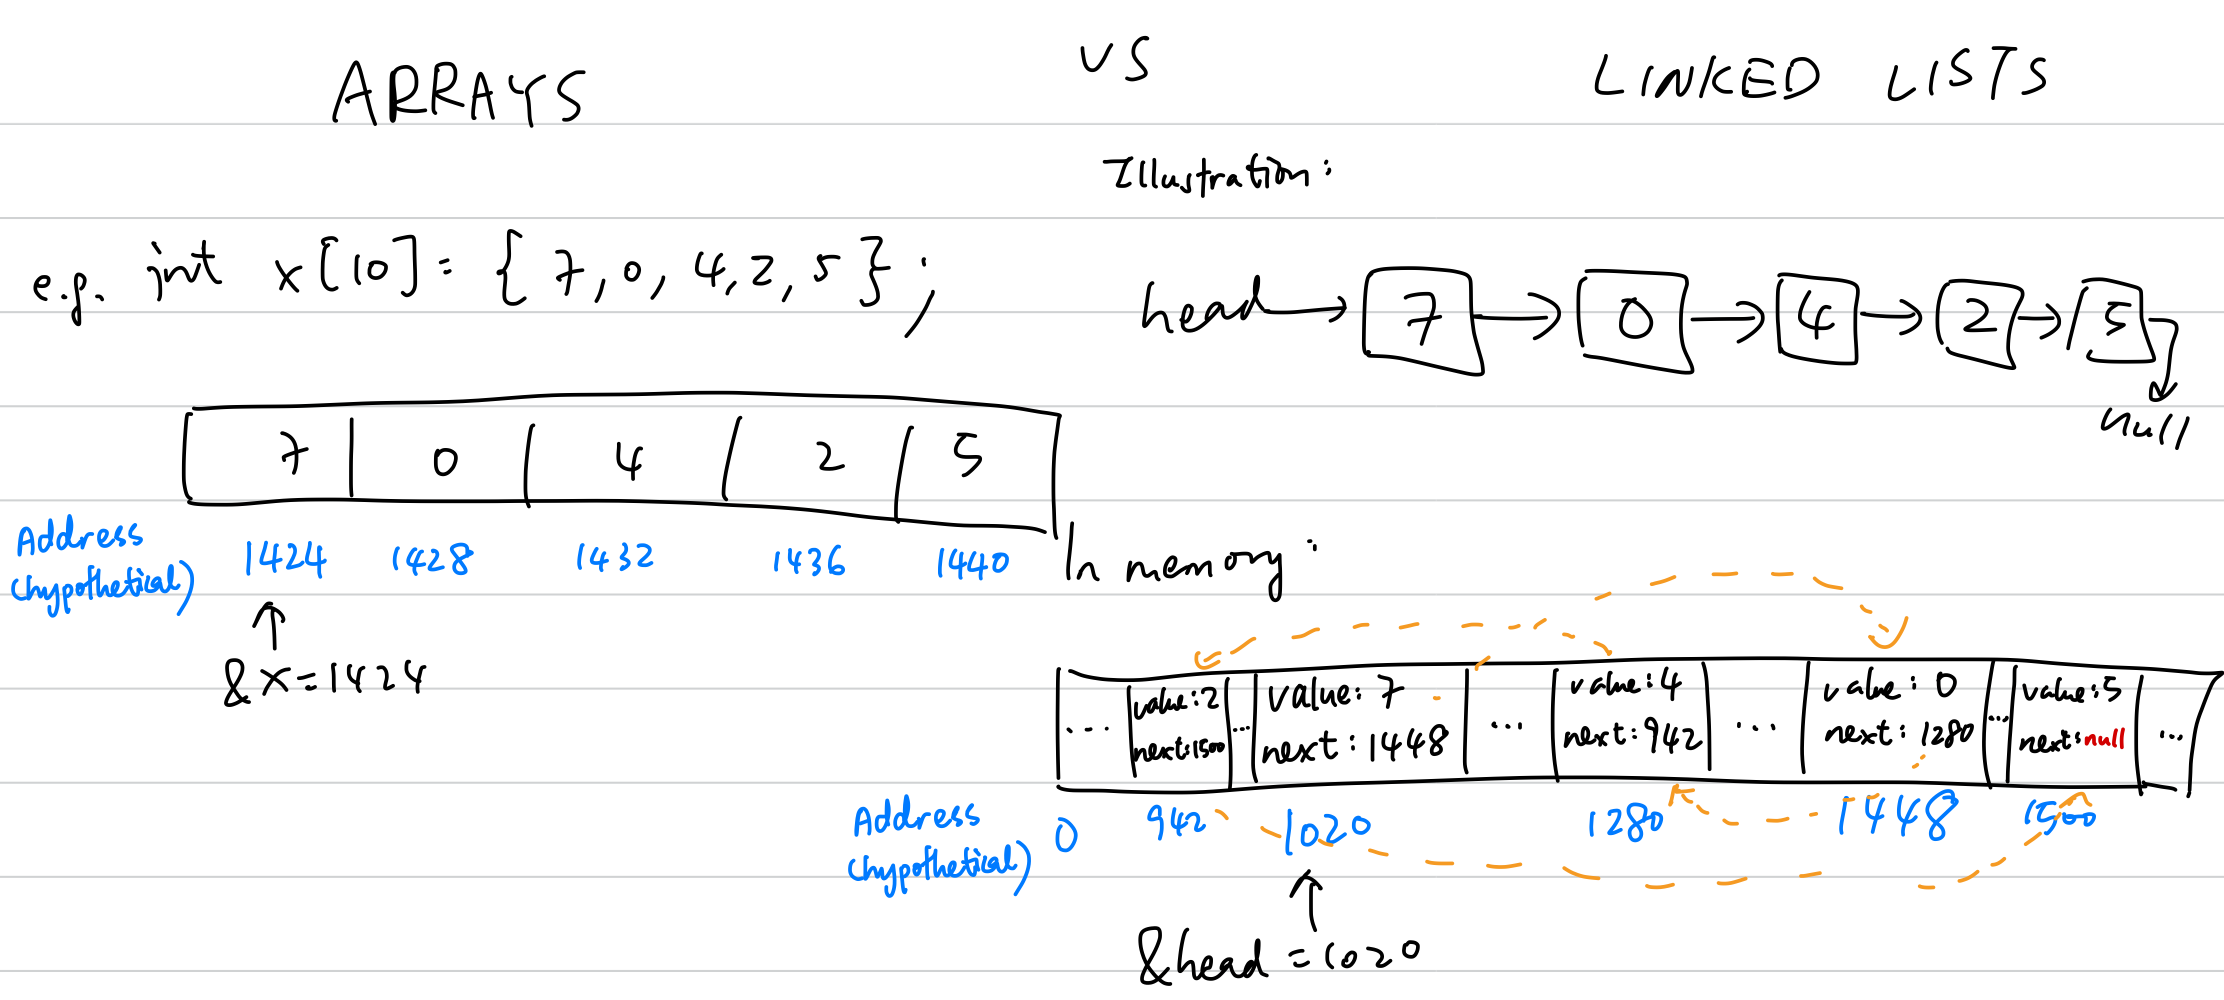
\includegraphics[width=15cm]{ch5-linkedlist1}

\subsection{Contrasting linked lists and arrays}

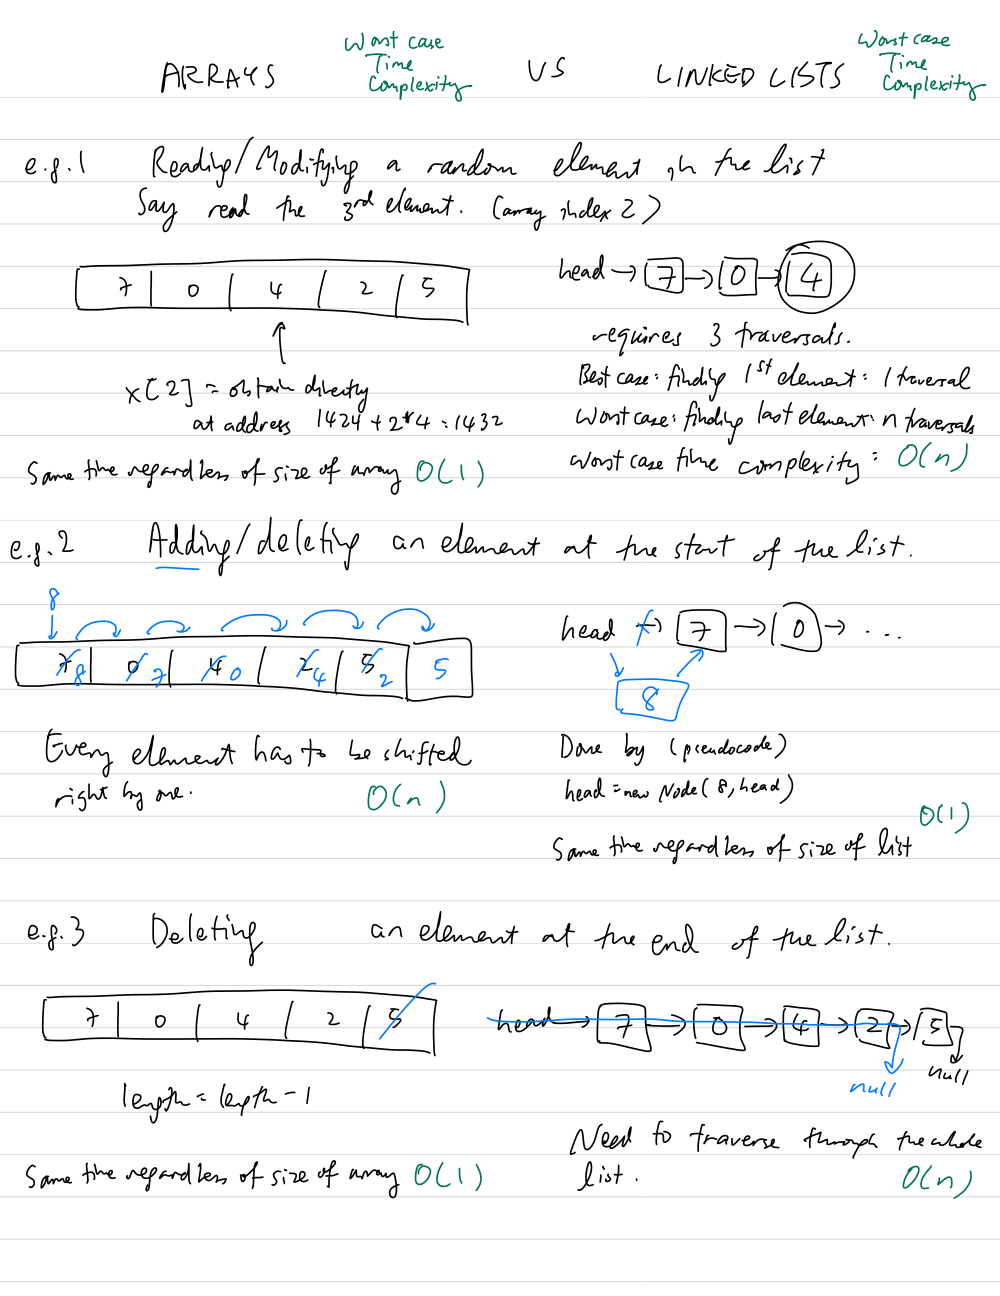
\includegraphics[width=15cm]{ch5-linkedlist2}

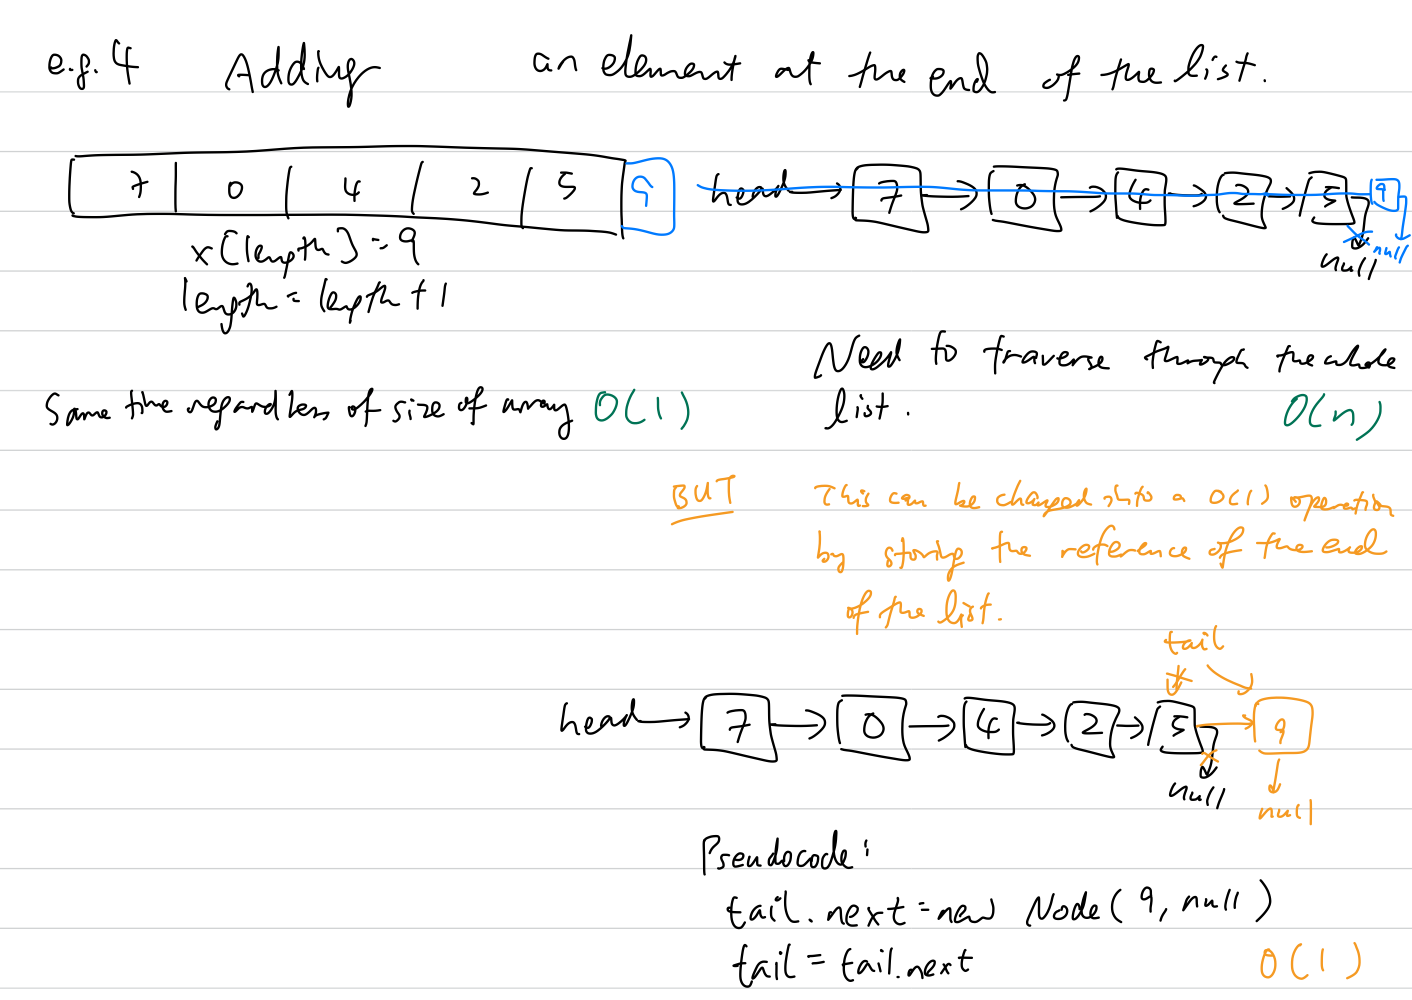
\includegraphics[width=15cm]{ch5-linkedlist3}

\section{Time complexity}
\label{sec:bigO}
You may noticed the weird symbols in green in the above table. This is what we call the \textbf{big-O notation}\index{big-O notation}. It is used to describe time complexity\index{time complexity}, that is how computational work needed scales as the problem scales in size. Work is usually measured in terms of number of copies, traversals, or comparisons, depending on what our aim actually is. Size is usually measured in terms of size of the array/ linked list.\footnote{There is a very rigorous mathematical definition to the big-O notation, but it is not required in understanding what it is.}

Some processes above have a time complexity of $O(1)$, that means the same amount of work is required no matter how long the array/ linked list is. This is fantastic news! 

While some other processes have a time complexity of $O(n)$, that means we have to do more work as the array/linked list lengthens, this is still manageable. 

Some other processes you will encounter in the next few chapters have a time complexity of $O(n^2)$, this is bad news, because the amount of work would quickly go out of hand as n grows.

You will also encounter $\log$\footnote{The logarithm function: $b^c = a$ then $log_b a = c$, where $b$ is the base} in the big-O notation. Don't be afraid, it is good news, because $\log n$ scales slower than n. When we describe big-O notation the log base can be ignored.

We will usually analyze the worst case time complexity, as we want to know about the weaknesses of the algorithms.\footnote{Out of scope: The best case time complexity is usually not meaningful, and it is difficult to analyze the average case time complexity because it is difficult to define 'average'}

\section{Conclusion}
As you can see, linked lists and arrays have different efficiencies when performing different operations. There is no 'better' data structure, it is the job of we computer scientists to figure out which data structure should be used based on the scenario. Both linked lists and arrays can be used to implement stacks and queues and the algorithms that I will mention in the coming chapters. 

Yet I do not advise you to code using linked lists in C++, in fact I will not do so in this piece of notes, because it is quite troublesome\footnote{Out of scope: It is possible in C++, as it includes some Object Oriented Programming (OOP) features, but without automatic garbage collecting and a large boilerplate for OOP, there are better languages to implement linked lists, like Java, Scala, or Python.
}.

\chapter{Stacks and Queues}

Stacks and queues are data structures, adapted from our daily life. We realized that we can implement stacks and queues using arrays or linked lists. We will look into them in this chapter. We will look at the concept on how to implement them efficiently and write C++ code for the array implementation.

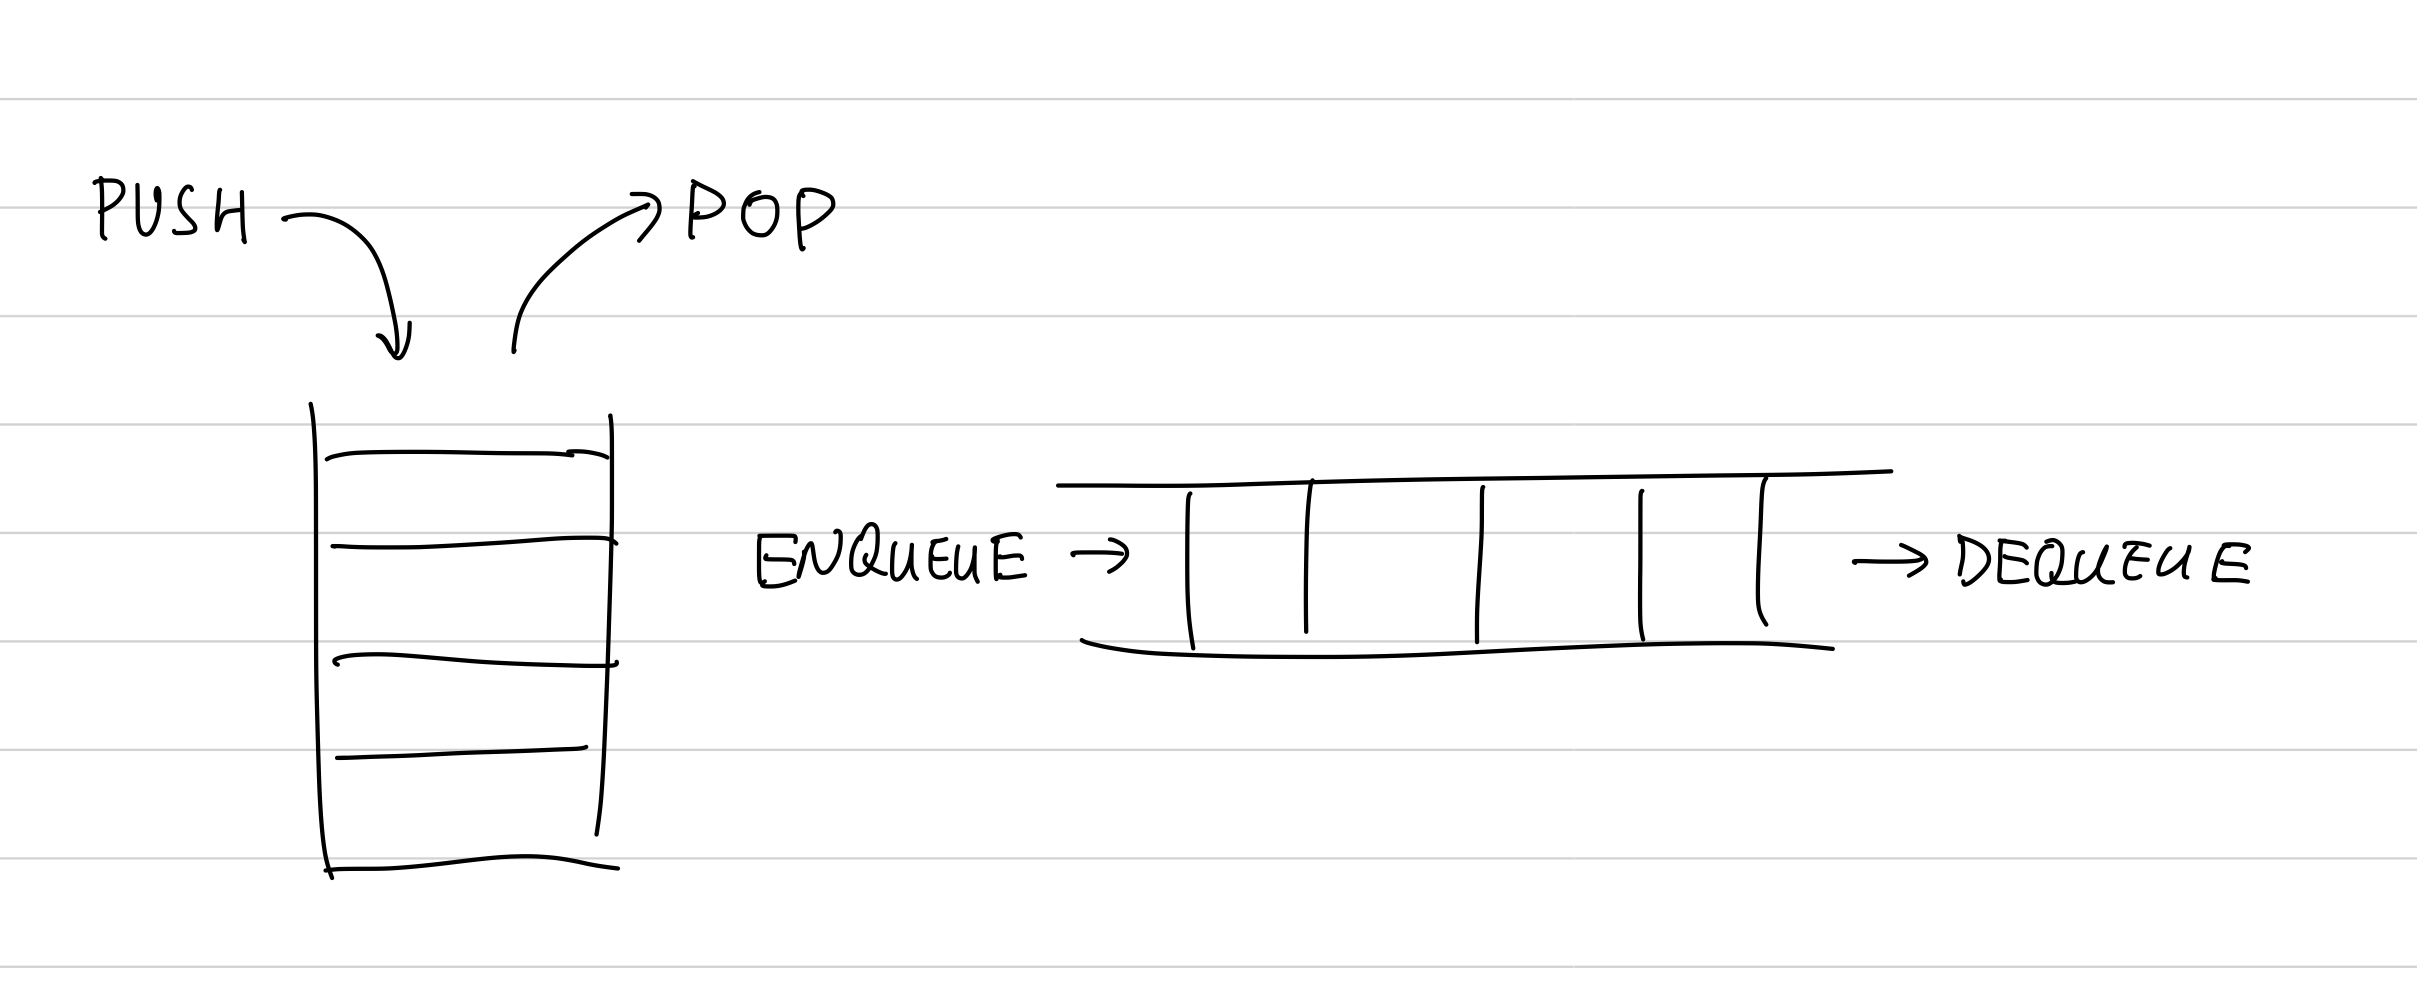
\includegraphics[width=15cm]{images/ch6-stackqueue.png}

\section{Further resources: mycodeschool}

Playlists by 
\href{https://www.youtube.com/user/mycodeschool}{mycodeschool}\footnote{Link: \href{https://www.youtube.com/user/mycodeschool}{https://www.youtube.com/user/mycodeschool}}
that focus on 
\href{https://www.youtube.com/watch?v=_OmRGjbyzno&list=PL2_aWCzGMAwLz3g66WrxFGSXvSsvyfzCO}{recursion}\footnote{Link: \href{https://www.youtube.com/watch?v=_OmRGjbyzno&list=PL2_aWCzGMAwLz3g66WrxFGSXvSsvyfzCO}{https://www.youtube.com/\\watch?v=\_OmRGjbyzno\&list=PL2\_aWCzGMAwLz3g66WrxFGSXvSsvyfzCO}}, 
\href{https://youtube.com/playlist?list=PL2_aWCzGMAwLZp6LMUKI3cc7pgGsasm2_}{pointers}\footnote{Link: \href{https://youtube.com/playlist?list=PL2_aWCzGMAwLZp6LMUKI3cc7pgGsasm2_}{https://youtube.com/playlist?list=PL2\_aWCzGMAwLZp6LMUKI3cc7pgGsasm2\_}} and 
\href{https://www.youtube.com/playlist?list=PL2_aWCzGMAwI3W_JlcBbtYTwiQSsOTa6P}{data structures (linked lists, stacks, queues)}\footnote{Link: \href{https://www.youtube.com/playlist?list=PL2_aWCzGMAwI3W_JlcBbtYTwiQSsOTa6P}{https://www.youtube.com/playlist?list=PL2\_aWCzGMAwI3W\_JlcBbtYTwiQSsOTa6P}}.
mycodeschool explains concepts about computing pretty well. You can watch his other playlists if interested.

\section{Stack}
Say you have a stack of towels put in a box, you would probably use the top towels first and make your way to the bottom, and you would also put new washed towels on the top. This is a stack, elements can only be inserted and removed at one end, what we call, \index{last in first out}(LIFO).

\begin{table}[h]
    \centering
    \begin{tabular}{|m{11em}|m{24em}|}
        \hline
        \textbf{Operations of a stack} & 
        Usage
        \\ \hline \hline
        
        \texttt{void push(int x)}\tablefootnote{It can store any other data types other than integers, however integer is selected for easier understanding, same applies to a lot of the algorithms discussed in the coming chapters} &
        Insert \texttt{x} to the top of the stack.
        \\ \hline
        
        \texttt{int pop()} &
        Remove the element at the top of the stack and return its value.
        \\ \hline
        
        \texttt{bool isEmpty()} &
        Returns \texttt{true} when the stack is empty, \texttt{false} otherwise.
        \\ \hline
        
        \texttt{int size()} &
        Return the current number of elements in the stack.
        \\ \hline
    \end{tabular}
\end{table}

Stacks can be easily implemented by both arrays and linked lists. As demonstrated by the illustrations. All processes should be done in $O(1)$ time.

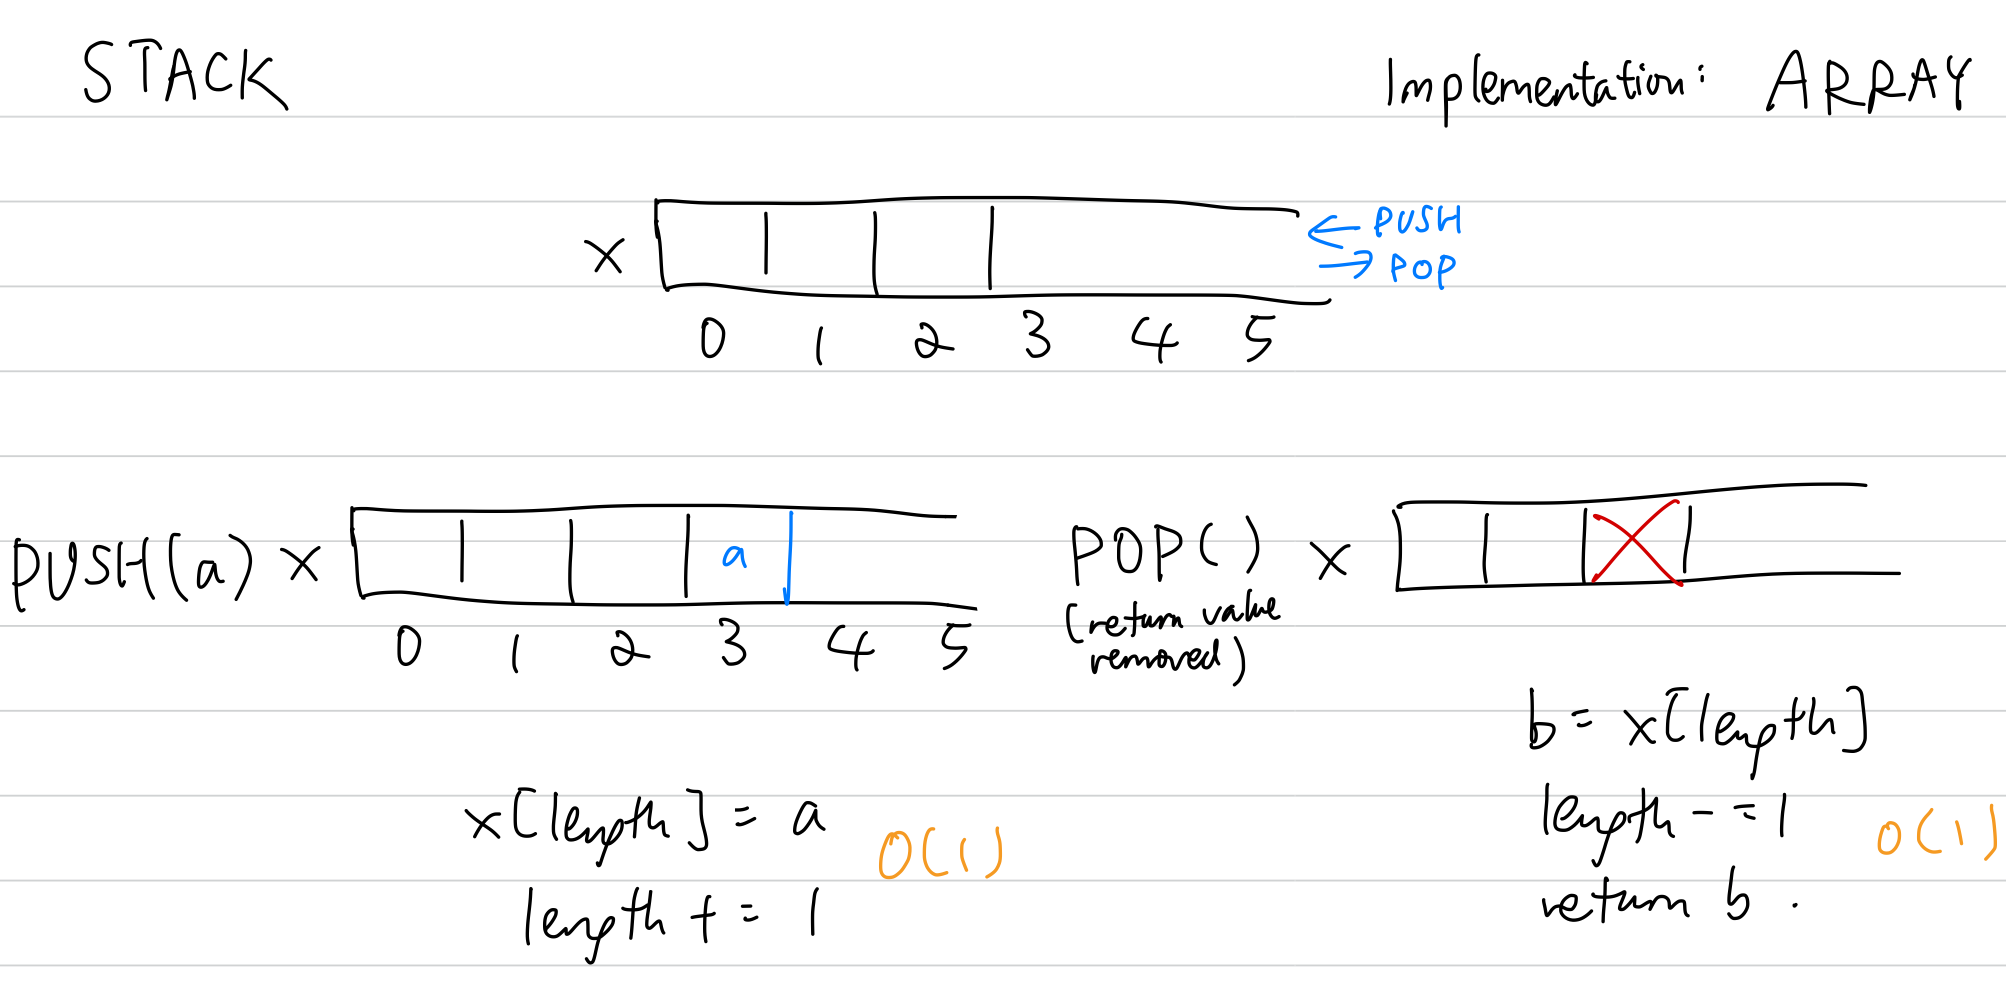
\includegraphics[width=15cm]{images/ch6-stackarray.png}

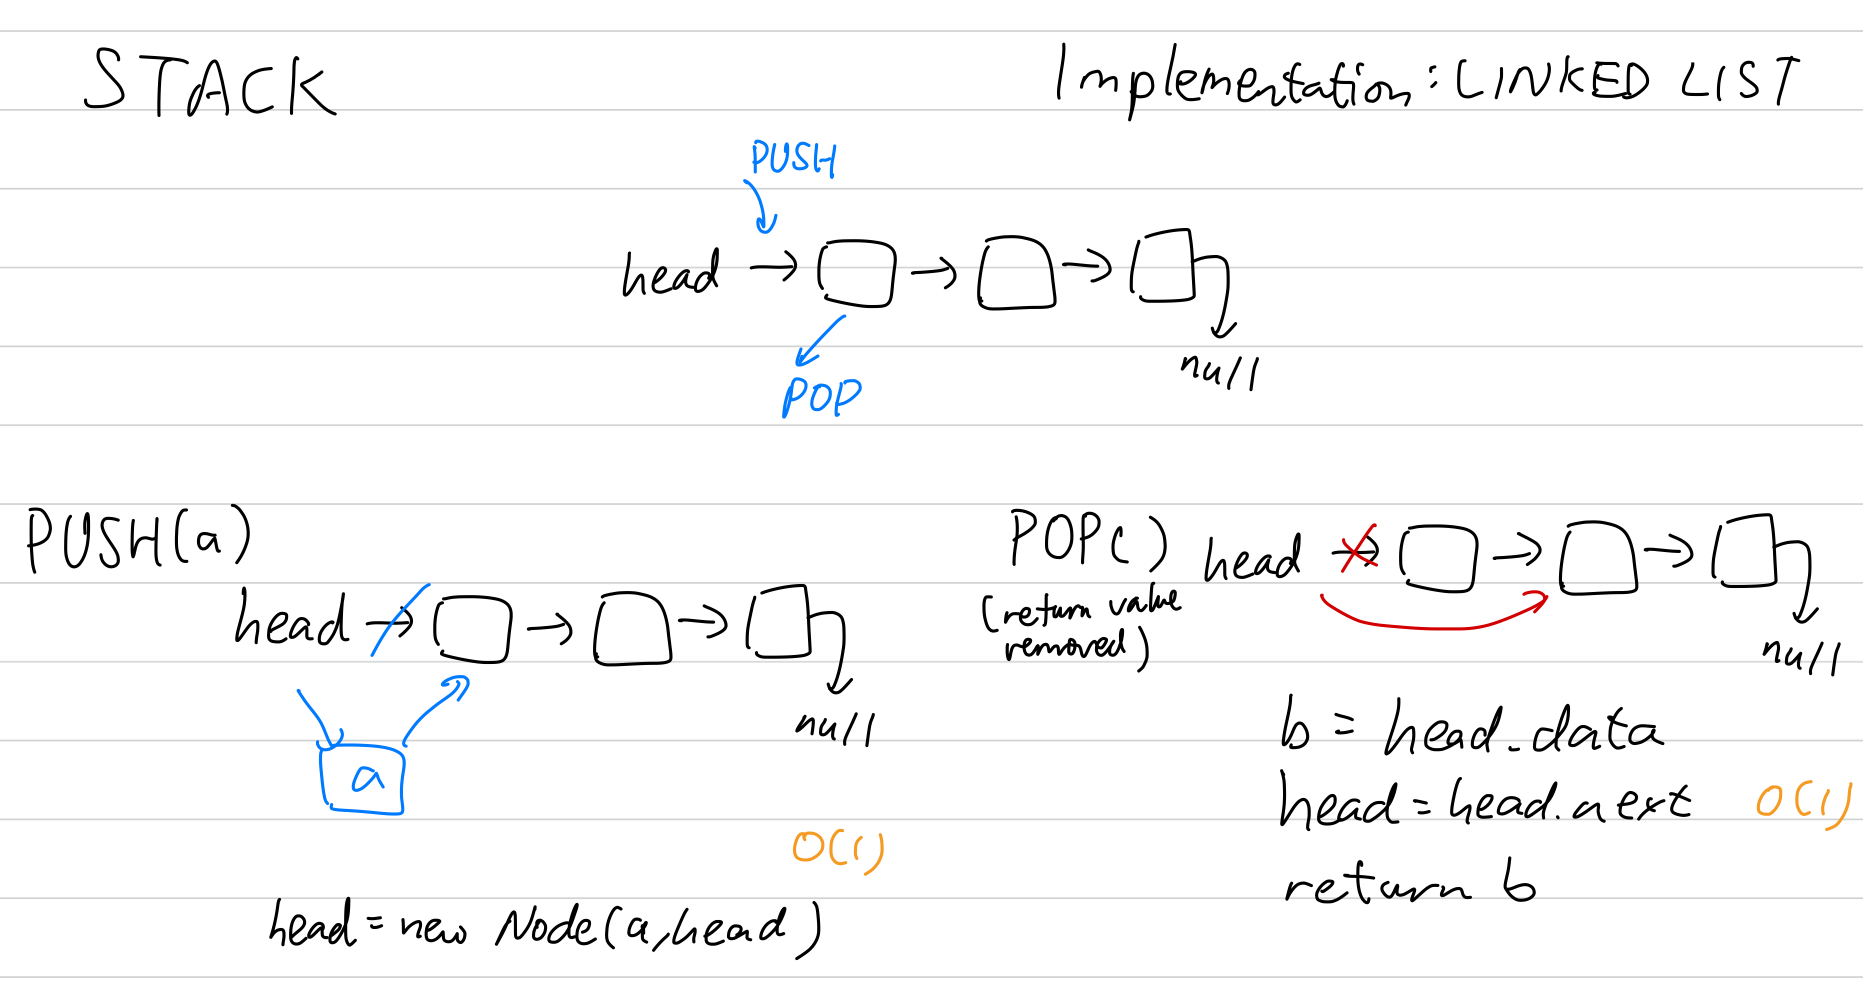
\includegraphics[width=15cm]{images/ch6-stacklinkedlist.png}

Let's look at the array implementation in code. In reality, array memory is limited, so we impose a MAX value and stop pushing elements when the stack is full.
\vspace{6mm}

C++: (\textit{Exercise: Try to re-implement yourself.})\footnote{The way to deal with the warnings when the stack is full/ empty depends on the use case. We will not cover it here.}
\begin{lstlisting}
const int MAX = 20; //can be larger
int stk[MAX] = {};
int _size = 0;

void push(int x){
    if(_size==MAX){ //what would happen if we remove this check?
        cout << "WARNING: Stack is full." << endl;
        return;
    }
    stk[_size] = x;
    _size++;
}

int pop(){
    if(_size==0){ //what would happen if we remove this check?
        cout << "WARNING: Stack is empty." << endl;
        return -1;
    }
    int x = stk[_size];
    _size--;
    return x;

    //alternatively: (less intuitive)
    // _size--;
    // return stk[_size+1];
}

int size(){ return _size;}

//Can we check whether the stack is empty by if(pop()==-1) instead?
bool isEmpty(){ return _size==0;}
\end{lstlisting}

Use example:
\begin{lstlisting}
int main(){
    cout << size() << " " << isEmpty() << endl; //0 1
    push(4);
    cout << size() << " " << isEmpty() << endl; //1 0
    push(5);
    cout << size() << " " << isEmpty() << endl; //2 0
    cout << pop() << endl; //5
    cout << size() << " " << isEmpty() << endl; //1 0
    cout << pop() << endl; //4
    cout << size() << " " << isEmpty() << endl; //0 1
    pop(); //WARNING: Stack is empty.
    cout << size() << " " << isEmpty() << endl; //0 1
} 
\end{lstlisting}
\section{Queue}
Just like a normal queue in daily life, people queue at one end and they are served when they reach the other end, what we call \index{first in first out} (FIFO).

\begin{table}[h]
    \centering
    \begin{tabular}{|m{11em}|m{24em}|}
        \hline
        \textbf{Operations of a queue} & 
        Usage
        \\ \hline \hline
        
        \texttt{void enqueue(int x)} &
        Insert \texttt{x} to one end of the queue.
        \\ \hline
        
        \texttt{int dequeue()} &
        Remove the element at the other end of the queue.
        \\ \hline
        
        \texttt{bool isEmpty()} &
        Returns \texttt{true} when the queue is empty, \texttt{false} otherwise.
        \\ \hline
        
        \texttt{int size()} &
        Return the current number of elements in the queue.
        \\ \hline
    \end{tabular}
\end{table}

Queues can be easily implemented by both arrays and linked lists. All processes should be done in $O(1)$ time.

Let's first focus on the array implementation:

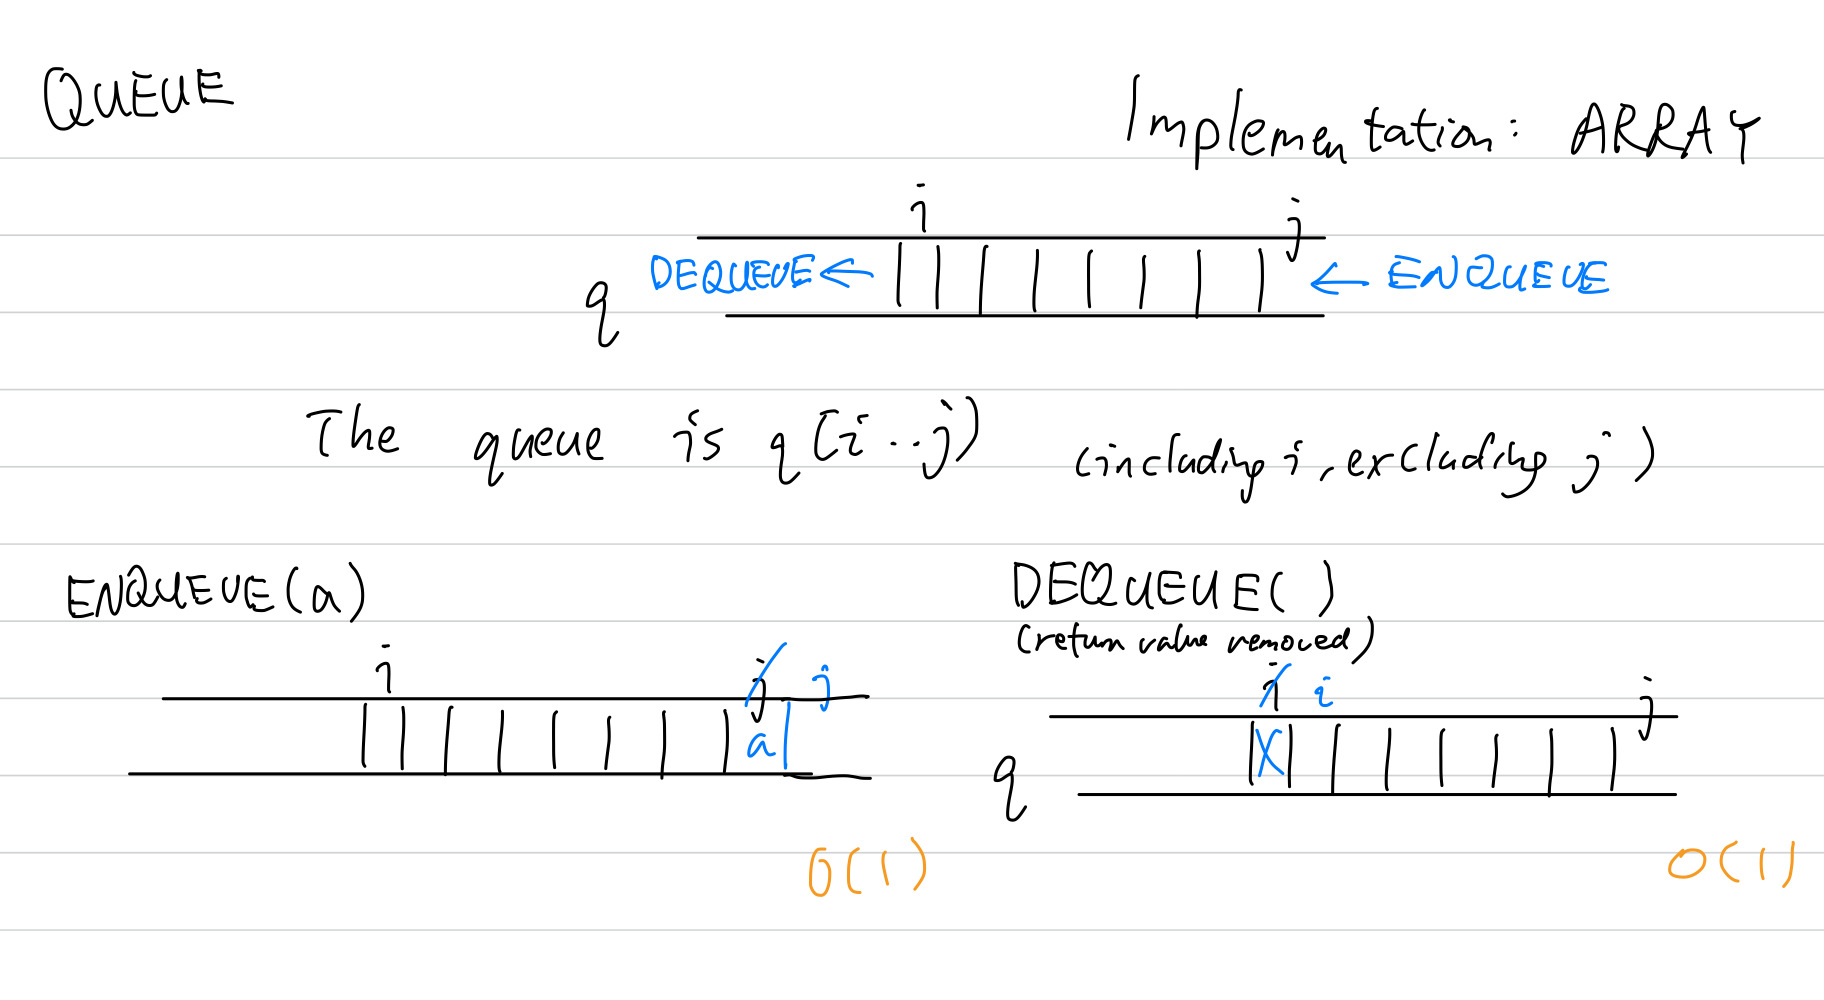
\includegraphics[width=14cm]{images/ch6-qarray.png}

Here is an implementation: \textit{(NOT the one you should follow)}

\begin{lstlisting}
//global variables, can be used by all functions
const int MAX = 20; //constants, cannot be changed throughout the program
int q[MAX] = {};
int i = 0;
int j = 0;
//The queue: q[i..j)

void enqueue(int x){
    if(j==MAX){
        cout << "WARNING: Queue is full." << endl;
        return;
    }
    q[j] = x;
    j++;
}

int dequeue(){
    if(i==j){
        cout << "WARNING: Queue is empty." << endl;
        return -1;
    }
    int x = q[i];
    i++;
    return x;
}

int size(){ return j-i;}

bool isEmpty(){ return i==j;}
\end{lstlisting}

Example usage:

\begin{lstlisting}
int main(){
    cout << size() << " " << isEmpty() << endl; //0 1
    enqueue(4);
    cout << size() << " " << isEmpty() << endl; //1 0
    enqueue(5);
    cout << size() << " " << isEmpty() << endl; //2 0
    cout << dequeue() << endl; //4
    cout << size() << " " << isEmpty() << endl; //1 0
    cout << dequeue() << endl; //5
    cout << size() << " " << isEmpty() << endl; //0 1
    dequeue(); //WARNING: Queue is empty.
    cout << size() << " " << isEmpty() << endl; //0 1
}
\end{lstlisting}

You can quickly see that there is a problem, variables \texttt{i} and \texttt{j} keep increasing but never decrease, eventually the queue cannot be used after \texttt{MAX} amount of insertions. This is unsustainable and we realized we can work around it.

The solution is a circular queue. Value of variables \texttt{i} and \texttt{j} circle round and round, going back to 0 after reaching \texttt{MAX-1}.

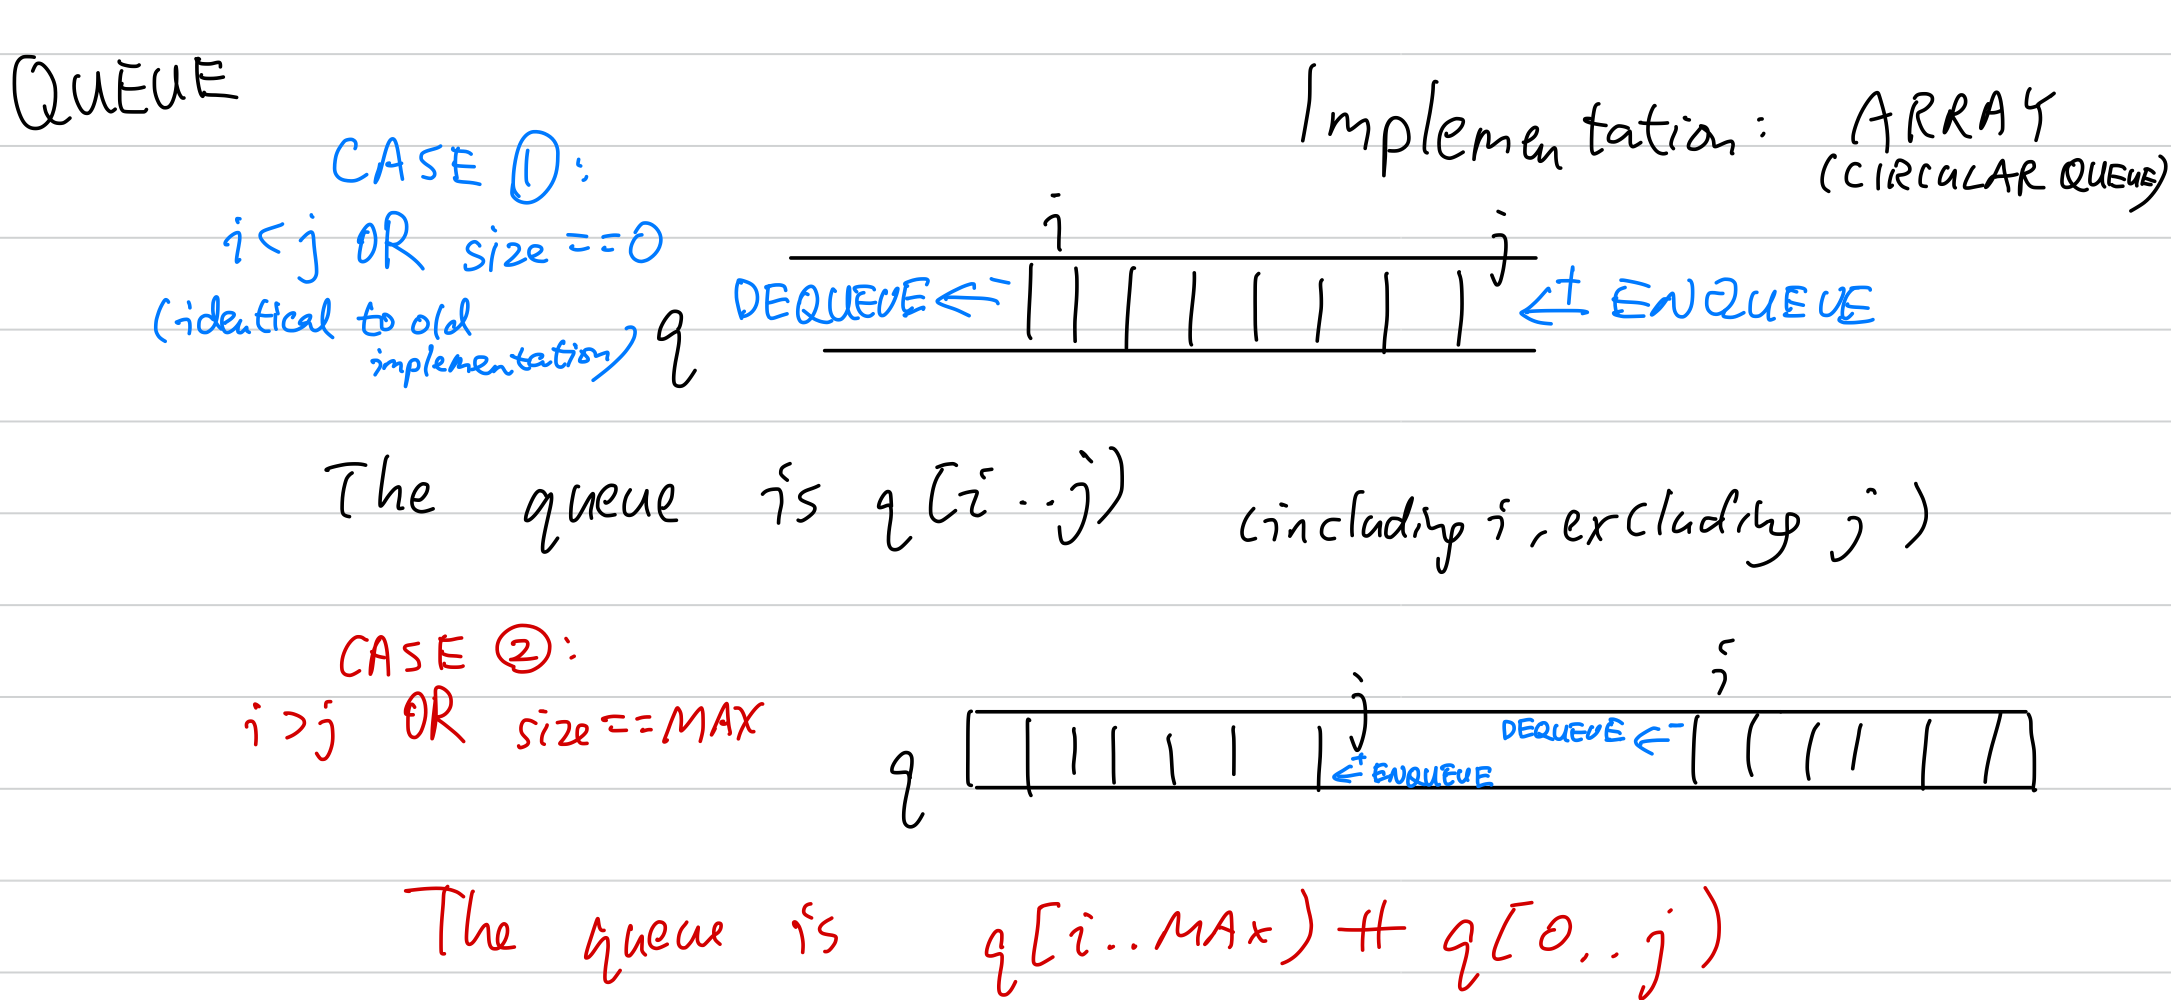
\includegraphics[width=14cm]{images/ch6-cq.png}

There is an ambiguity when \texttt{i=j}, it can either mean the queue is completely full, or the queue is completely empty. One solution is to introduce a \texttt{size} variable, to keep track of the size and differentiate the two cases.

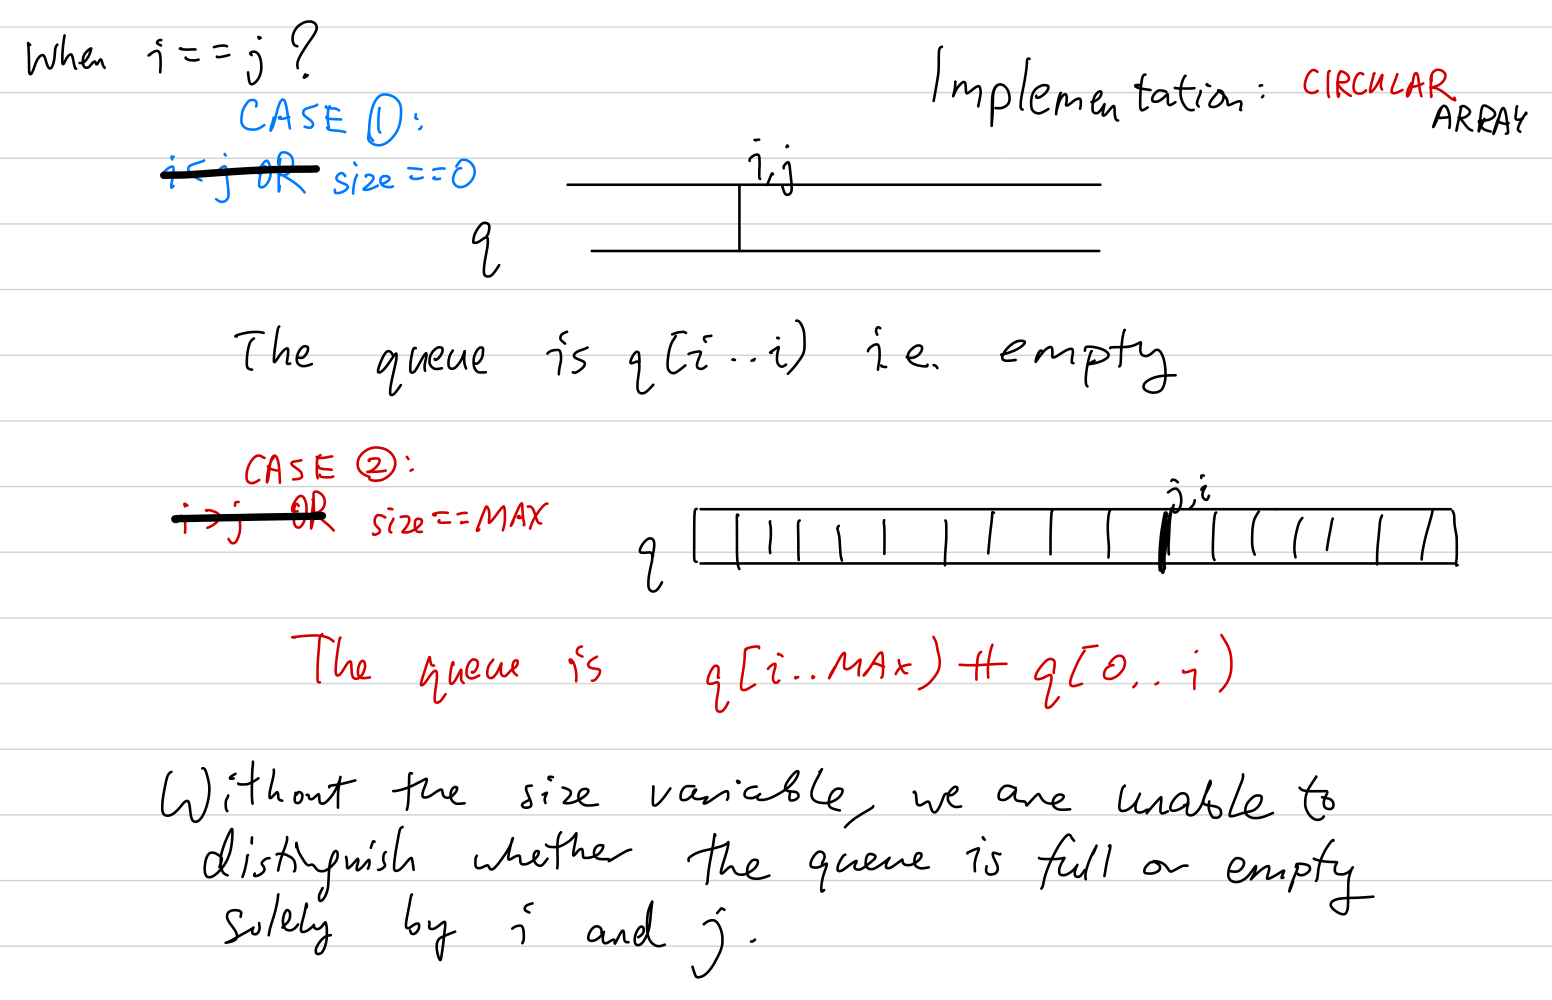
\includegraphics[width=14cm]{images/ch6-cqij.png}

C++: \textit{(Exercise:  Try to re-implement yourself.)}

\begin{lstlisting}
const int MAX = 20; 
int cq[MAX] = {};
int i = 0;
int j = 0;
int _size = 0;

void enqueue(int x){
    if(_size==MAX){
        cout << "WARNING: Queue is full." << endl;
        return;
    }
    cq[j] = x;
    j = (j+1)%MAX;
    _size++;
}

int dequeue(){
    if(_size==0){
        cout << "WARNING: Queue is empty." << endl;
        return -1;
    }
    int x = cq[i];
    i = (i+1)%MAX;
    _size--;
    return x;
}

int size(){ return _size;}

bool isEmpty(){ return _size==0;}
\end{lstlisting}
\vspace{6mm}

Finally, the outline of the linked list implementation:

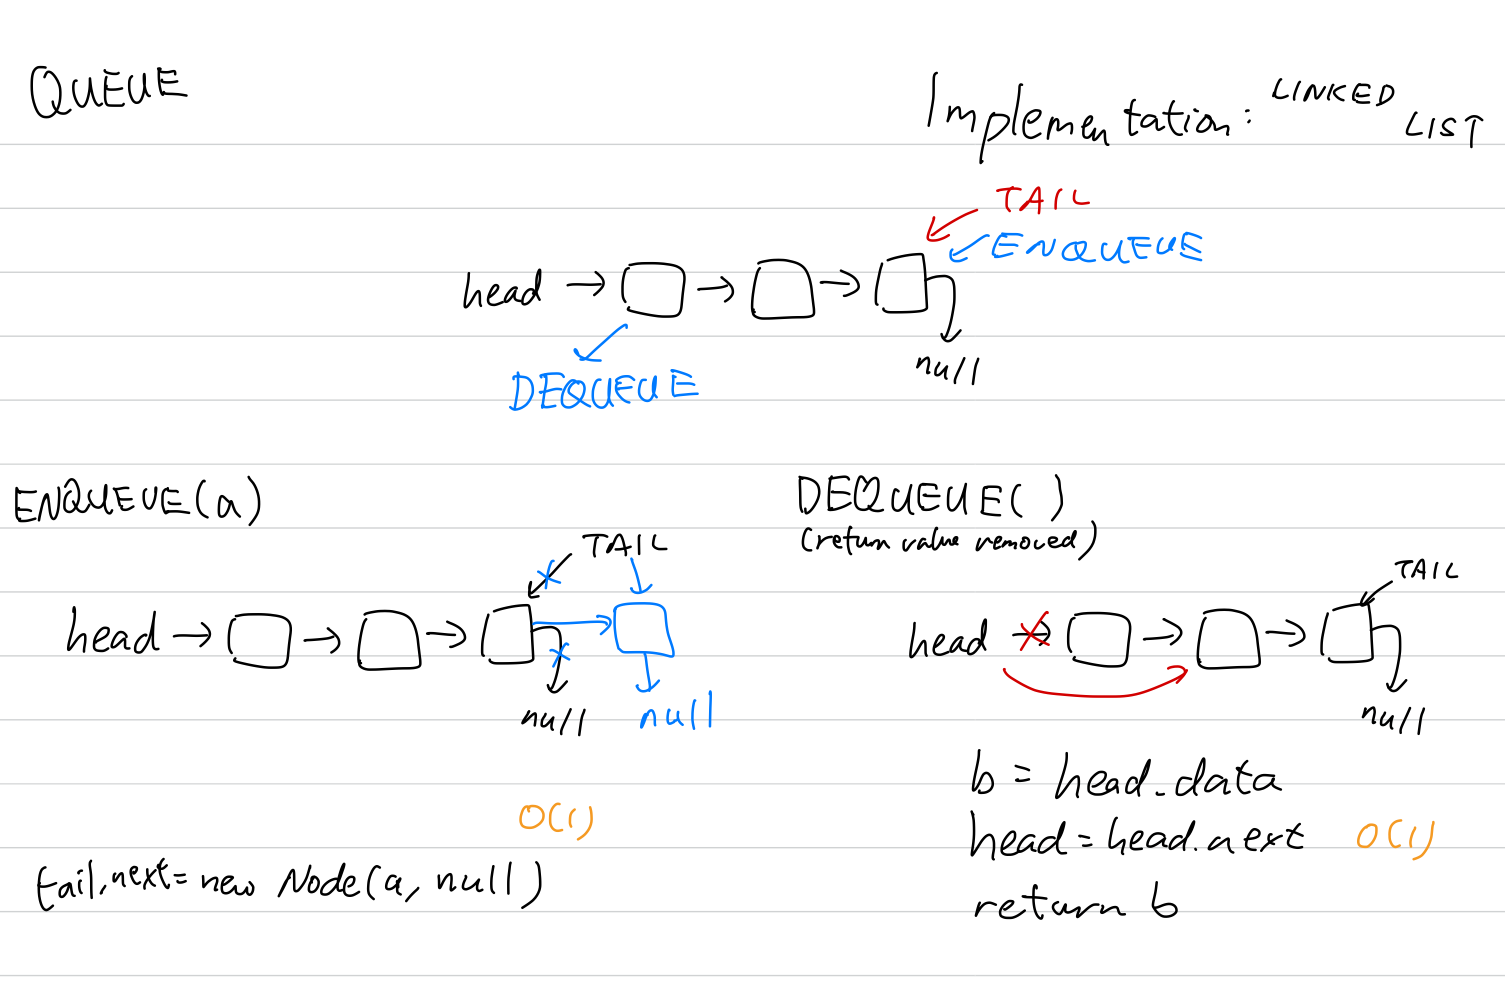
\includegraphics[width=14cm]{images/ch6-qlinkedlist.png}
\chapter{Searching Algorithms}

In this chapter we will look into some algorithms that search for a specific integer in an array, and return its index in the array. We will look at how they work and analyze their efficiency (using time complexity). We will only focus on implementation using arrays.

\section{Further resources}

Watching animations of these algorithms is useful in understanding how they work. Algorithms in this and the next chapter are all very famous, I am sure you can find plenty of them online.

\section{Linear search}

Linear search works with all arrays, it returns the location of the leftmost occurrence of the integer when there are duplicates, and returns \textit{n} if the integer is not found.

\begin{lstlisting}
int main(){
    int x[] = {3,1,4,1,5,9,2,6};

    cout << linearSearch(x,8,1) << endl; //1 (leftmost occurance)
    cout << linearSearch(x,8,2) << endl; //6
    cout << linearSearch(x,8,7) << endl; //8 (not found, return n)
}
\end{lstlisting}

It might not be completely clear whether the target is in the array or not, but have to check by:

\begin{lstlisting}
int i = linearSearch(x,8,target);
if(i<n)
    cout << target << " found at location " << i << endl;
else 
    cout << target << " not found" << endl;
\end{lstlisting}

Now, after we have clarified what it does, let's implement it in C++.
\vspace{6mm}

C++: (\textit{Exercise: Try to re-implement yourself.})
\begin{lstlisting}
int linearSearch(int x[], int n, int target){
    int i = 0;
    while(i<n){
        if(x[i]==target) break;
        i++;
    }
    return i;
}
\end{lstlisting}

If you want to eliminate the \texttt{break} statement, you could replace the loop by:

\begin{lstlisting}
while(i<n&&x[i]!=target) i++;
//can we change the order of the tests?
\end{lstlisting}

Time complexity: O(n) comparisons
\vspace{6mm}

The worst case occurs when the target is not found or the target is the last element, the while loop is run \textit{n} times to search through the whole array before returning.

\pagebreak

\section{Binary search}

In fact, we can do better. Yet this requires the array to be \textbf{sorted} beforehand.

Every time we can cut the array in half, and compare the target with the middle element (x[m]). Let's say the segment that the target might be in is x[i..j) (including i and excluding j). We try to maintain that structure that the right hand index is always excluded, and the left hand index is always included, to avoid complications of code.
\vspace{6mm}

If x[m] $<$ target, we know all elements with index $<=$ m are also smaller than the target, because the array is sorted. We can set the lower boundary to m+1.

If x[m] $>$ target, we know all elements with index $>=$ m are also larger than the target, because the array is sorted. We can then set the upper boundary to m. (excluding m)

In either case, around half of the array is eliminated from consideration.

Process continues when the target is found (x[m] = target).
\vspace{6mm}

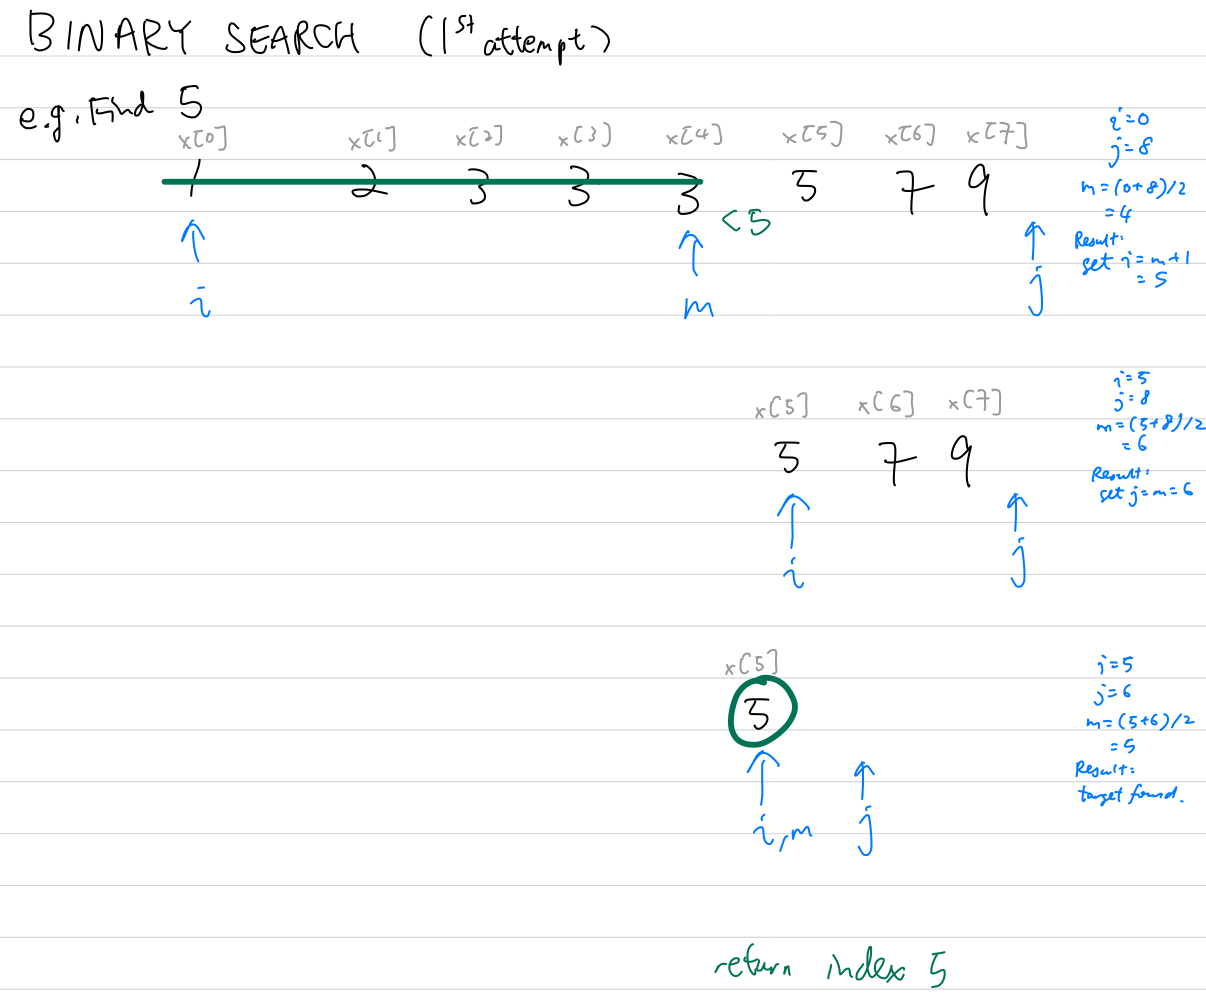
\includegraphics[width=14cm]{images/ch7-binarysearch1.png}
\pagebreak

Here is an implementation: \textit{(NOT the one you should follow)}

\begin{lstlisting}
int binarySearch1(int x[], int n, int target){
    int i=0;
    int j=n;
    while(i<j){
        //array segment: x[i..j)
        //stopping condition is i=j because the array would be empty
        int m = (i+j)/2;
        if(x[m]<target){
            //new array segment: x[m+1..j)
            i = m+1;
        }else if(x[m]>target){
            //new array segment: x[i..m)
            j = m;
        }else{
            //a match is found
            return m;
        }
    }
    return -1; //not found
}

int main(){
    int x[] = {1,2,3,3,3,5,7,9};

    cout << binarySearch1(x,8,1) << endl; //0 
    cout << binarySearch1(x,8,2) << endl; //1
    cout << binarySearch1(x,8,7) << endl; //6

    //there are multiple 3s, should it return 2,3 or 4? Is it consistent?
    cout << binarySearch1(x,8,3) << endl; //4

    //4 is not in the array, can it return something more meaningful other than -1?
    cout << binarySearch1(x,8,4) << endl; //-1
}
\end{lstlisting}

\pagebreak

\subsection*{To be precise}

How about duplicate targets in the array? To maintain consistency, we should return the location of the leftmost occurrence of the target. 

How about targets that are not found in the array? We should return the location where the target can be inserted to maintain the order of the array. 

To achieve these goals, we have to change our concept slightly. (Surprisingly these changes lead to neater code)

We will imagine that we split the array into three sections, x[0..i) contains all elements that are checked $<$ target, x[i..j) contains all elements that are not checked yet, and x[j..n) contains all elements that are checked $>=$ target. 

We maintain this relationship from start to finish. Initially, we set i=0, j=n, so that the first and the last sections are empty signifying all elements are unchecked. Then we gradually check the elements using binary search (similar to the concept explained in the previous section), until i=j, meaning that all elements are checked. Then we return a value.
\vspace{6mm}

Which value shall we return? If the value is present, x[0..i) contains all elements that $<$ target, and x[i..n)\footnote{remember i=j when binary search terminates} contains all elements that $>=$ target. 

If the target is present, it will be at location i. If there are duplicates, the leftmost occurrence will be at location i. If the target is not present. The proper location to insert it is also location i. So i should be returned regardless. Neat!

Followed are some illustrations that further elaborate on the concept, and also the implementation in C++.
\vspace{6mm}

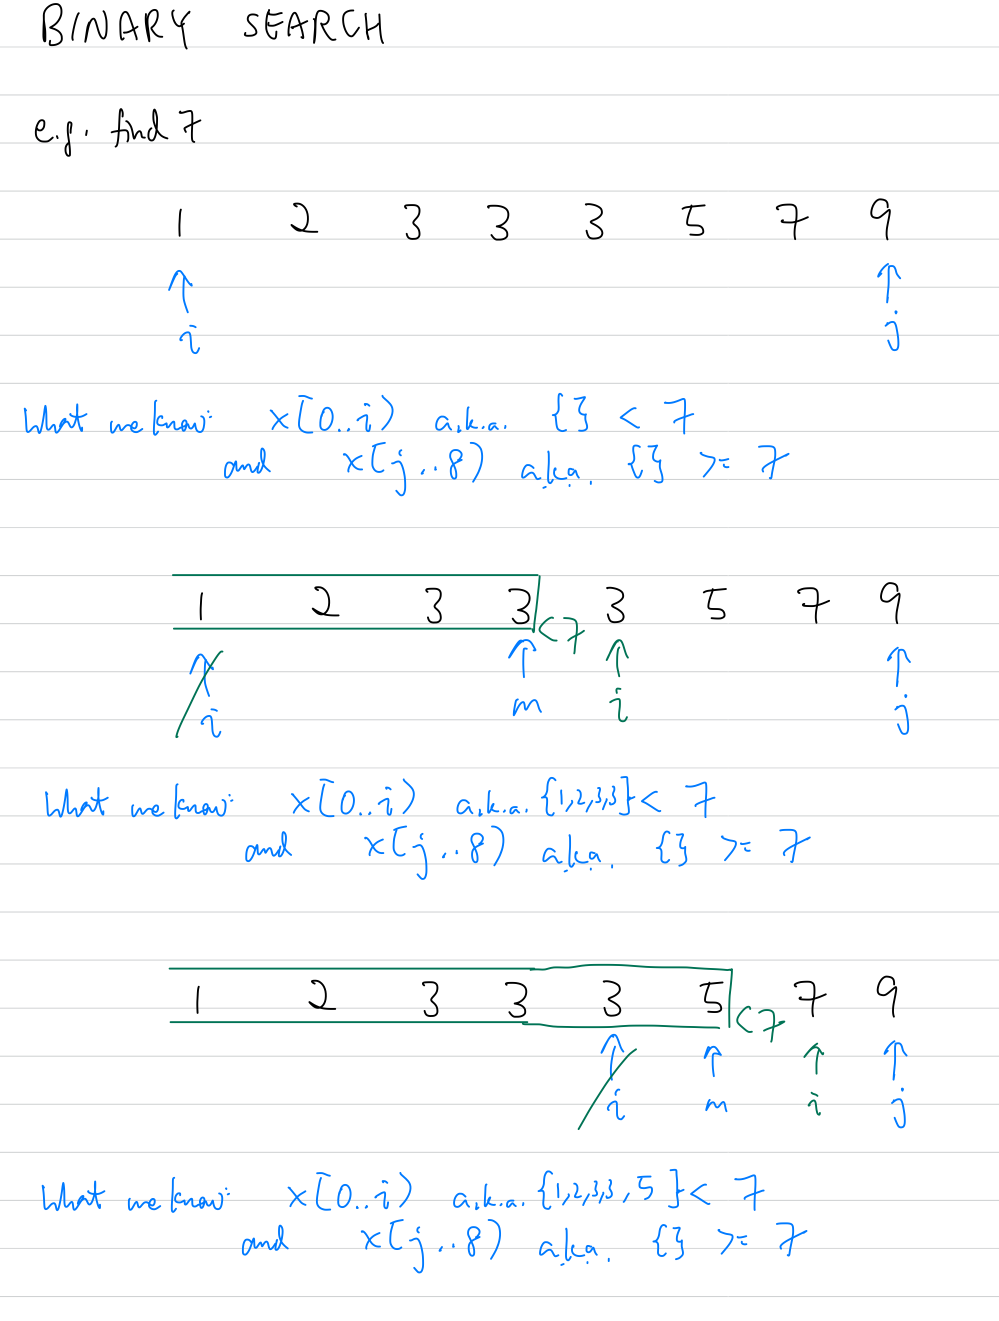
\includegraphics[width=12.5cm]{images/ch7-binarysearch71.png}

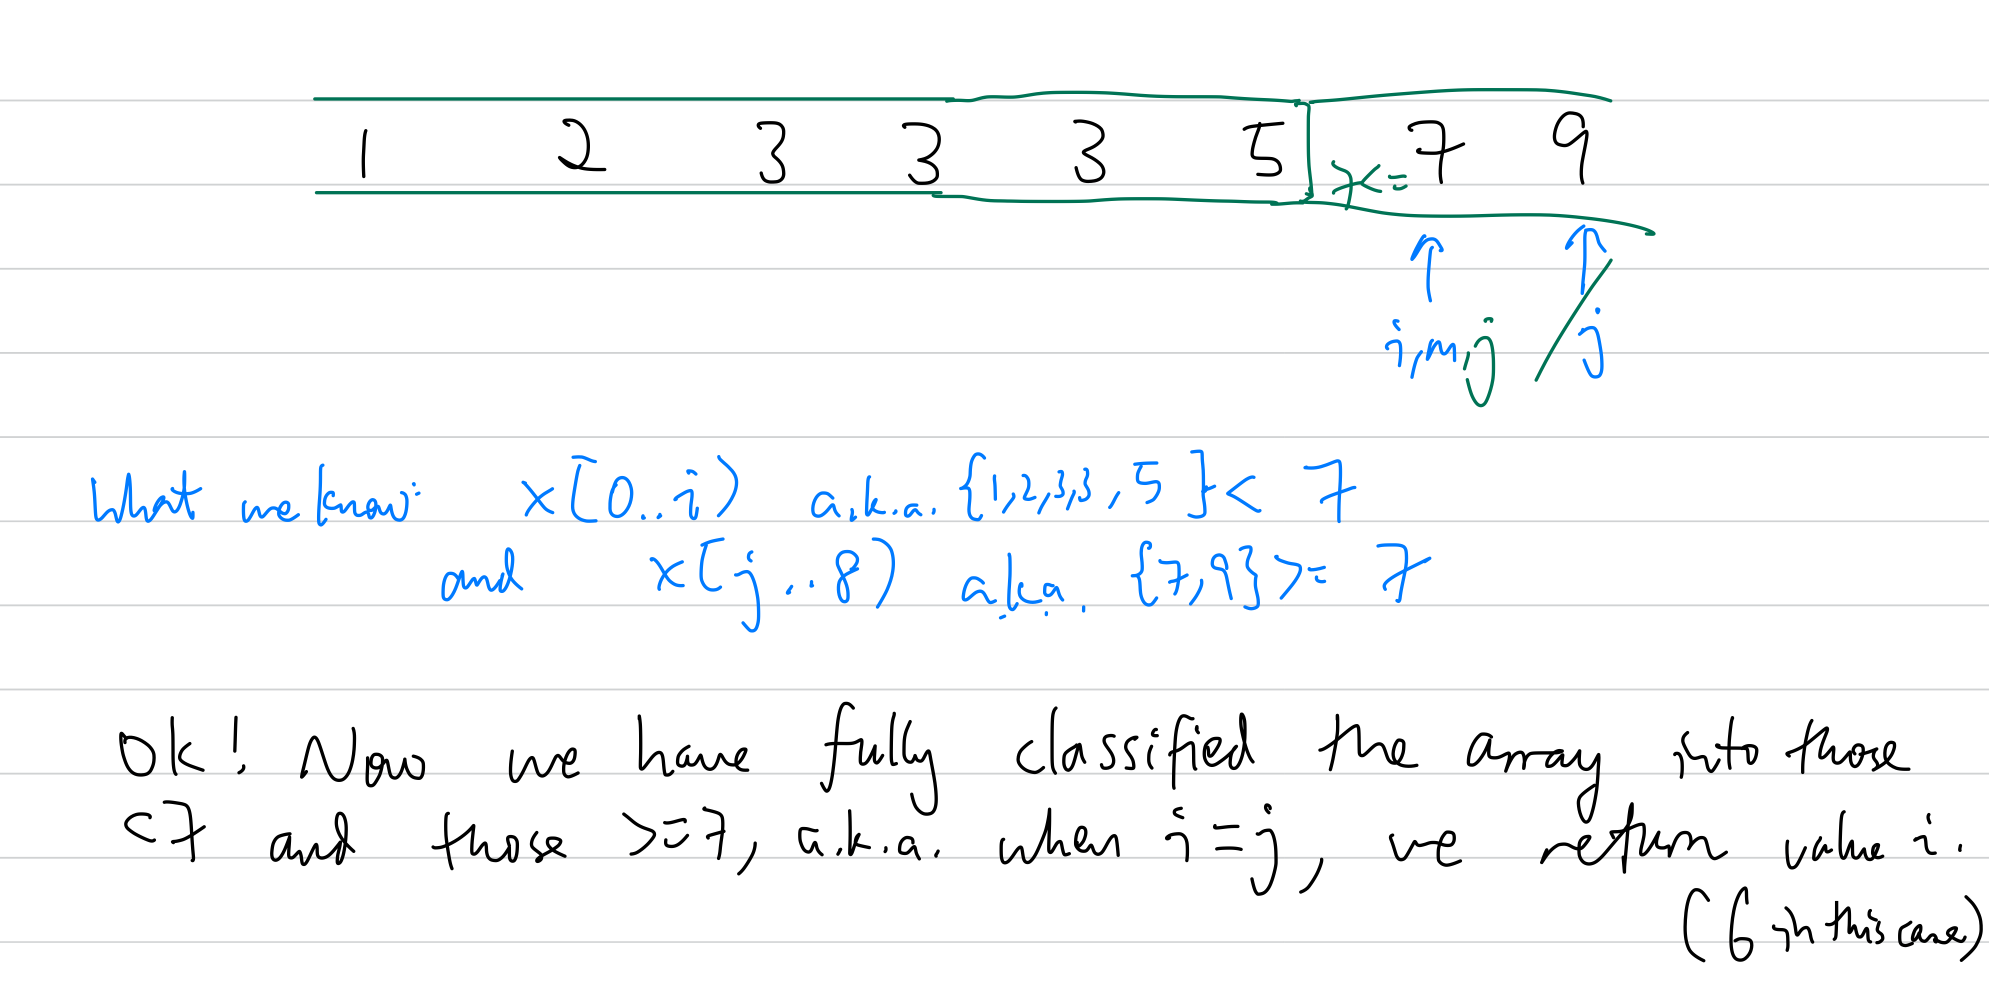
\includegraphics[width=12.5cm]{images/ch7-binarysearch72.png}

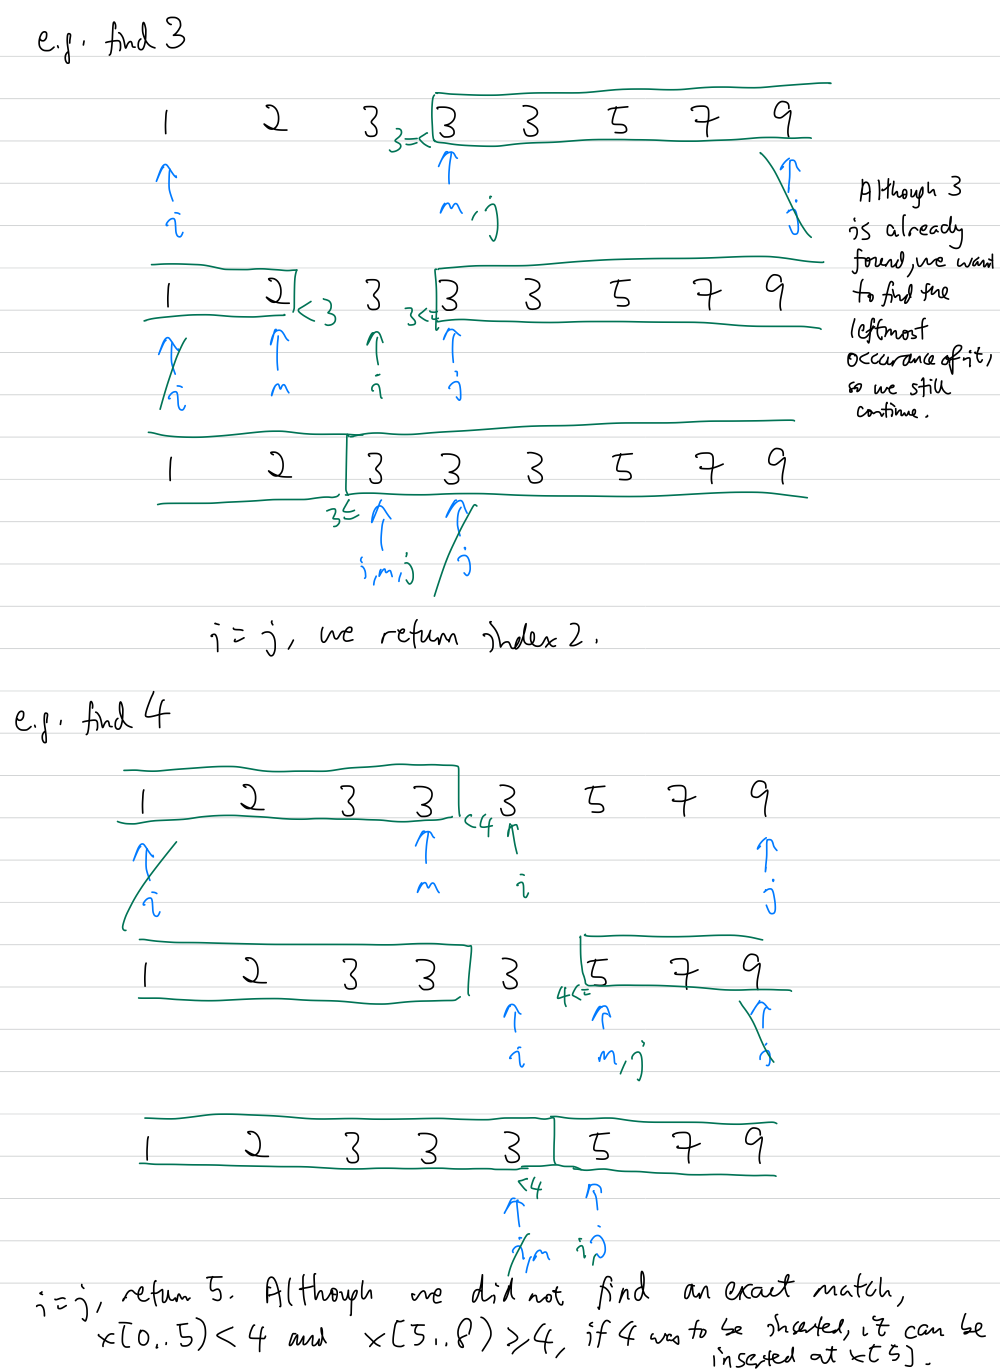
\includegraphics[width=14cm]{images/ch7-binarysearch34.png}

\pagebreak

C++: \textit{(Exercise:  Try to re-implement yourself.)}

\begin{lstlisting}
int binarySearch(int x[], int n, int target){
    int i=0;
    int j=n;
    while(i<j){
        //array segment: x[i..j)
        int m = (i+j)/2;
        if(x[m]<target){
            //new array segment: x[m+1..j)
            i = m+1;
        }else {
            //new array segment: x[i..m)
            j = m;
        }
    }
    return i;
}

int main(){
    int x[] = {1,2,3,3,3,5,7,9};

    cout << binarySearch(x,8,1) << endl; //0 
    cout << binarySearch(x,8,2) << endl; //1
    cout << binarySearch(x,8,7) << endl; //6

    cout << binarySearch(x,8,3) << endl; //2 (leftmost occurance)

    cout << binarySearch(x,8,4) << endl; //5 (the index that number 4 should be inserted)
}
\end{lstlisting}

It might not be completely clear whether the target is in the array, but we could easily check by:

\begin{lstlisting}
int i = binarySearch(x,8,target);
if(i<n && x[i]==target) //Is i<n necessary? Can we change the order of the tests?
    cout << target << " found at location " << i << endl;
else 
    cout << target << " not found, it can be inserted at location " << i << endl;
\end{lstlisting}

Time complexity: $O(\log n)$ comparisons
\vspace{6mm}

In each step, around half of the array is eliminated from consideration. Each step takes constant time.

\section{Conclusion}

\begin{table}[h]
    \centering
    \begin{tabular}{|m{6em}|m{9em}|m{18em}|}
        \hline  
        \textbf{Searching Algorithms} & 
        \multicolumn{2}{l|}{Goal: Find location of target in an array}
        \\ \hline \hline
        
        Algorithm &
        Time Complexity & 
        Remarks
        \\ \hline \hline
        
        Linear search &
        $O(n)$ &
        Works for all arrays
        \\ \hline
        
        Binary search &
        $O(\log n)$ &
        Works only for sorted arrays, much faster
        \\ \hline
    \end{tabular}
\end{table}

Binary search should be used when the data is sorted (which is commonly the case), linear search otherwise.
\chapter{Sorting Algorithms}

In this chapter we will look at some algorithms that sort an array of integers\footnote{The algorithms also work for other data types with linear order defined. However integer is selected for easier understanding.} of length \textit{n} in ascending order. We will look at how they work and analyze their efficiency (using time complexity). We will only focus on implementation using arrays.

To demonstrate different sorting algorithms, we would use this code right here as a template to verify whether the algorithms work:

\begin{lstlisting}
#include <iostream>
using namespace std;
int main(){
    int x[] = {3,1,4,1,5,9,2,6};
    
    //the sorting function accepts the array and the length of the array, this is common practice, as it is impossible to determine the length of the array in C/C++ when only the array is given.
    sort(x,8); //replace with name of the sorting function

    //print everything in x, with commas properly placed
    //check if the answer is 1,1,2,3,4,5,6,9
    cout << x[0];
    for(int i = 1; i < 8;  i++){
        cout << "," << x[i];
    }
    cout << endl;
}
\end{lstlisting}
\pagebreak
\section{Bubble sort}

Bubble sort swaps the places of two adjacent integers when it realizes they are out of order, until all integers are all sorted.

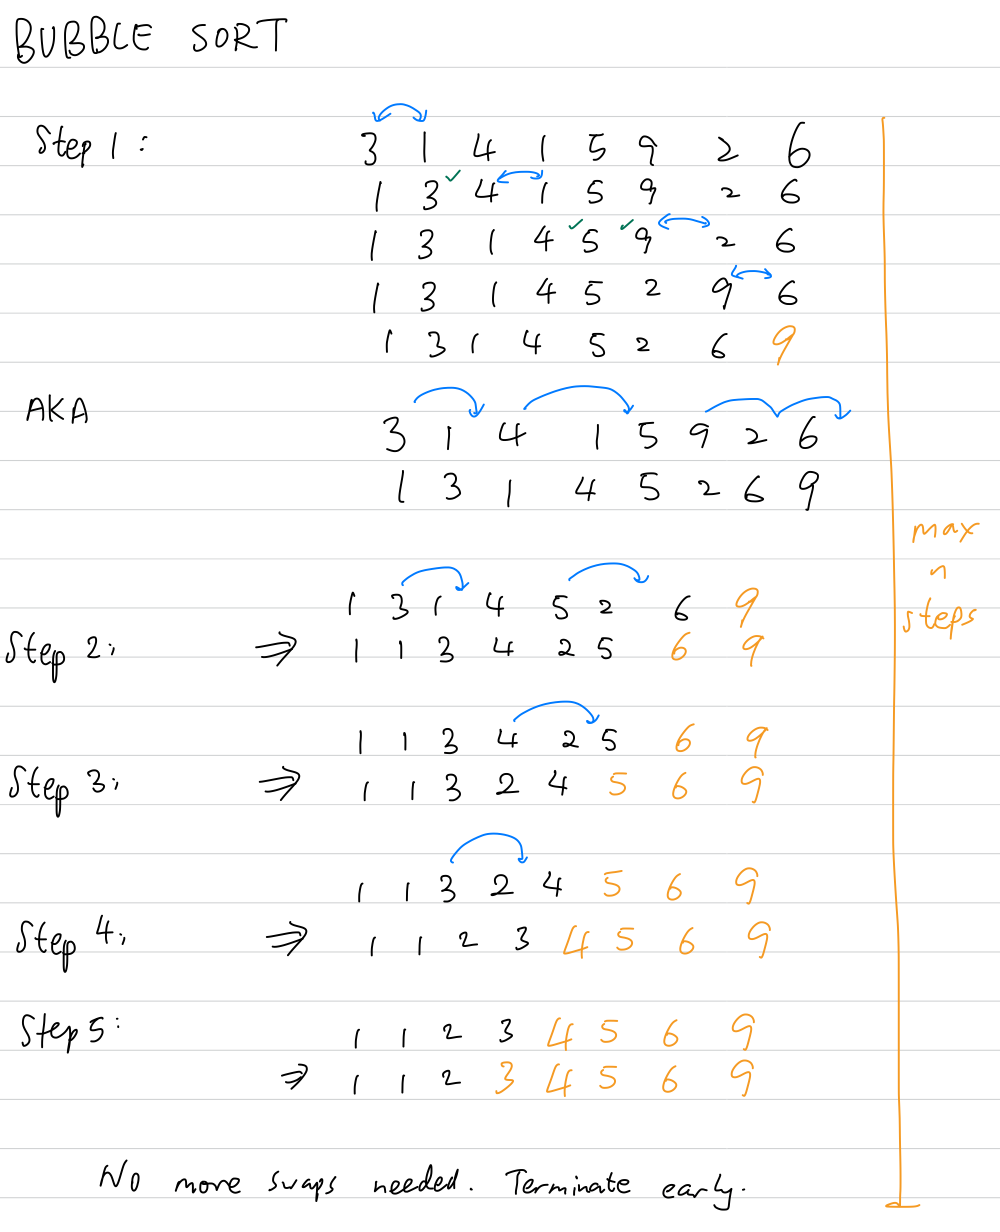
\includegraphics[width=15cm]{ch8-bubblesort.png}

\pagebreak

% Pseudocode:
% \begin{lstlisting}[language=Python,basicstyle=\rmfamily]
% bsort(x,n):
%     while(not sorted):
%         for j from 0 to n-1:
%             if x[j] > x[j+1]:
%                 swap(x[j],x[j+1]
% \end{lstlisting}

\pagebreak

At the \textit{i}th iteration of the outer loop, the last \textit{i} elements of the array are put at their sorted location. To guarantee the array is sorted, the inner loop is run \textit{n} times.
\vspace{6mm}

C++: (\textit{Exercise: Try to re-implement yourself.})
\begin{lstlisting}
void bsort(int x[], int n){
    for(int i = 0; i < n; i++){
        for(int j = 0; j < n-i-1; j++){ //the last i elements are sorted, no need to loop again
            if(x[j]>x[j+1]){
                int temp = x[j];
                x[j] = x[j+1];
                x[j+1] = temp;
            }
        } 
    }
}
\end{lstlisting}

Time complexity: $O(n^2)$ comparisons
\vspace{6mm}

There are \textit{n} steps, each step involves checking and swapping data from start to finish, taking time proportional to \textit{n} (in the worst case).

\pagebreak

\section{Selection sort}

Selection sort selects the minimum element and put it in front of the sorted array. Repeats until all elements are extracted.

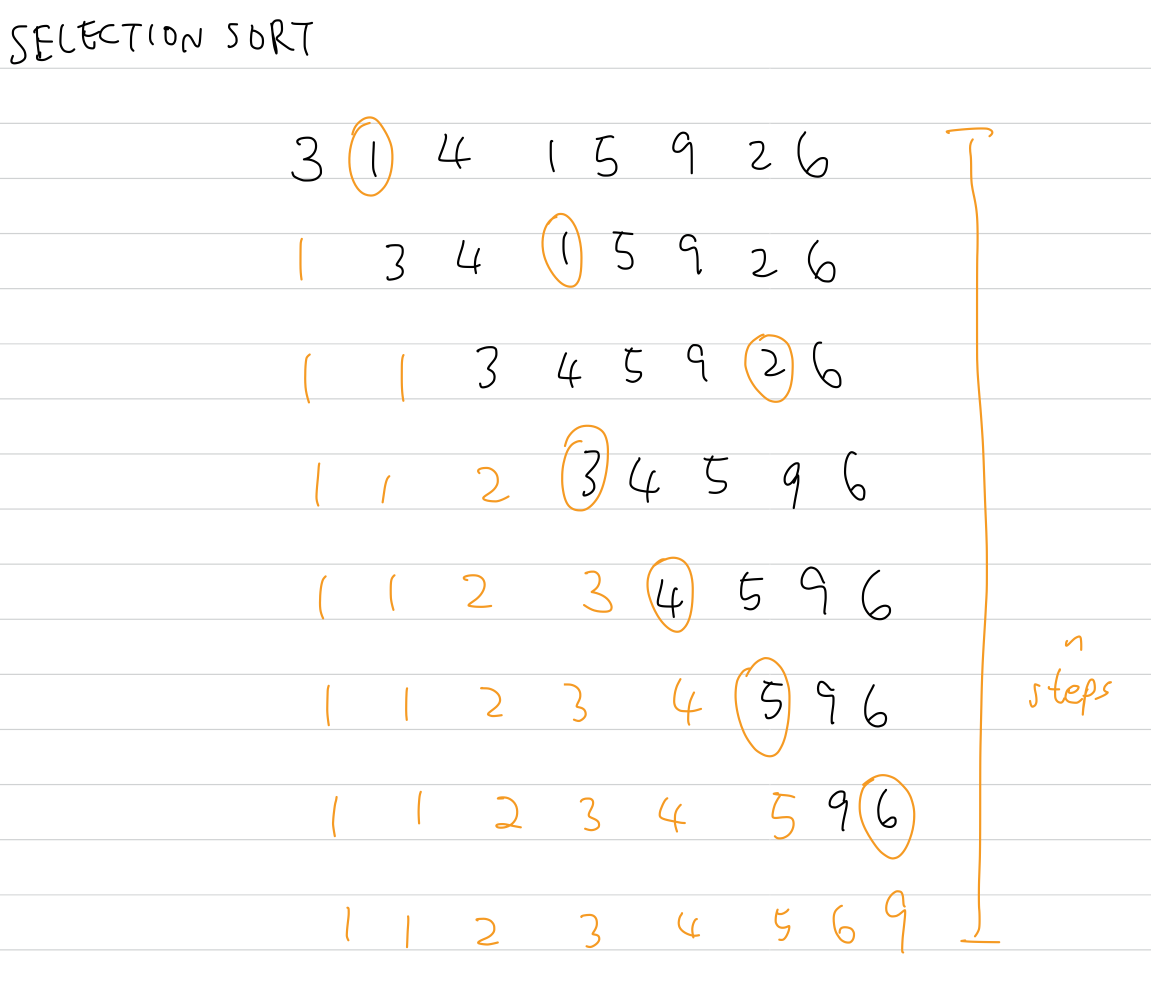
\includegraphics[width=16cm]{ch8-selectionsort.png}

\pagebreak

% Pseudocode:
% \begin{lstlisting}[language=Python,basicstyle=\rmfamily]
% ssort(x,n):
%     y = []
%     for each element in array x:
%         i = select-minimum(x) //get index of minimum element in x
%         y.append(x[i]) //add this element to the back of the newly created array
%         x.remove(i) //remove that minimum element from consideration
%     return y
% \end{lstlisting}

\pagebreak

C++: (\textit{Exercise: Try to re-implement yourself.})
\begin{lstlisting}
void ssort(int x[], int n){
    for(int i=0; i<n; i++){
    
        //find minimum value and its index in the array
        int minValue = x[i]; //Can we put 0 here instead?
        int minIndex = i;
        for(int j=i; j<n; j++){
            if(minValue > x[j]){
                minValue = x[j];
                minIndex = j;
            }
        }
        
        //swap x[i] with x[minIndex]
        x[minIndex] = x[i];
        x[i] = minValue;        
    }
}
\end{lstlisting}

Time complexity: $O(n^2)$ comparisons
\vspace{6mm}

There are \textit{n} steps, each step involves finding the minimum value, taking time proportional to \textit{n}.

\pagebreak

\section{Insertion sort}

Insertion sort assumes the leftmost element is a sorted array, then slowly adds elements in one by one, preserving the order of the sorted array.

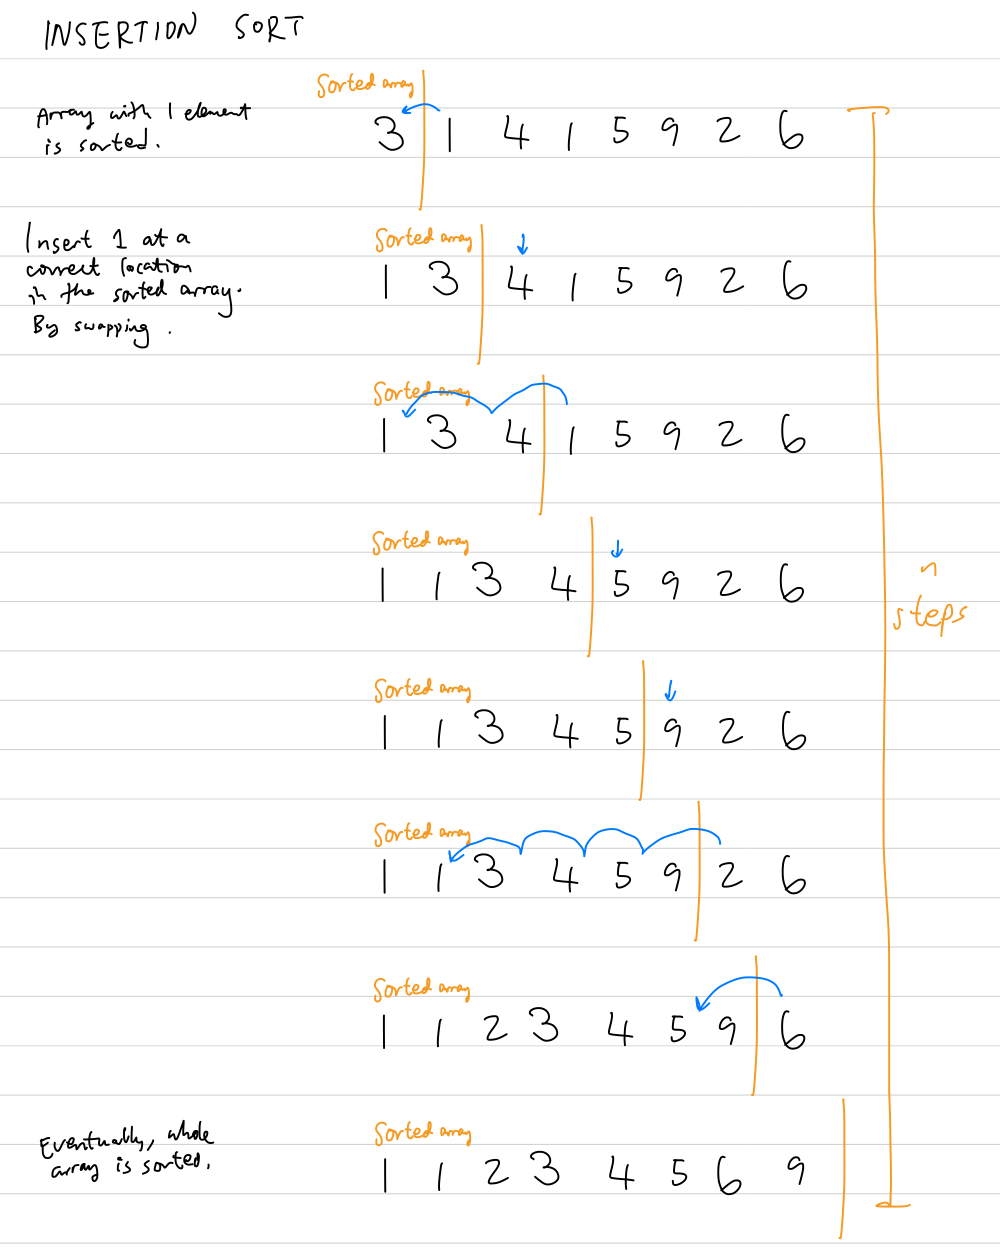
\includegraphics[width=15cm]{ch8-insertionsort.png}


% Pseudocode:
% \begin{lstlisting}[language=Python,basicstyle=\rmfamily]
% isort(x,n):
%     for i from 1 to n:
%         insert(x,i,x[i])

% insert(x,i,v):
%     j = i-1
%     while(j>0 and x[j] > v){
%         x[j+1] = x[j]
%         i--
%     }
%     x[j] = v
% \end{lstlisting}
% \vspace{6mm}
\pagebreak

C++: (\textit{Exercise: Try to re-implement yourself.})
\begin{lstlisting}
void isort(int x[], int n){
    for(int i=1; i<n; i++){
        int j = i-1;
        while(j>=0&&x[j] > x[j+1]){
            int temp = x[j];
            x[j] = x[j+1];
            x[j+1] = temp;
            j--;
        }
    }
}
\end{lstlisting}

Time complexity: $O(n^2)$ comparisons
\vspace{6mm}

There are \textit{n} steps, each step involves finding the correct location to insert the value concerned, taking time proportional to \textit{n}.

\pagebreak

\section{Merge sort}

Merge sort first splits the array repeatedly until all arrays are of length 1, where they are sorted without any actions. Then it merges back them two by two in order, eventually we get back the whole array in sorted order.

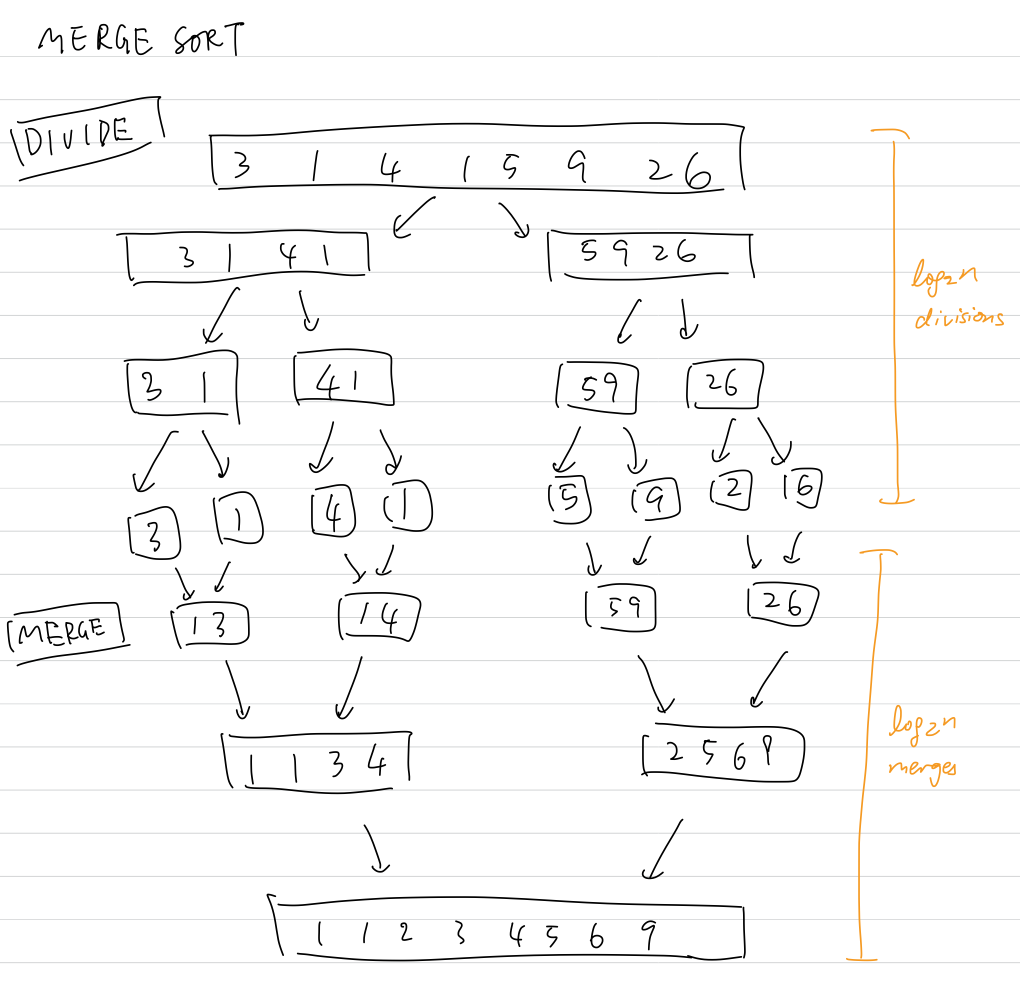
\includegraphics[width=15cm]{ch8-mergesort.png}

\pagebreak

% Pseudocode:
% \begin{lstlisting}[language=Haskell,basicstyle=\rmfamily]
% msort(x) = merge(msort(l),msort(r))
%     where l = first half of x, r = second half of x
% msort({}) = {}
% msort({a}) = {a} 

% merge(a,b)
%     | null a: b
%     | null b: a
%     | head a <= head b : [head a] ++ merge(tail a, b)
%     | else: [head b] ++ merge(a, tail b)
% \end{lstlisting}
% \vspace{6mm}

C++: (\textit{Exercise: Try to re-implement yourself.})

Call by \texttt{msort(x,0,8);}

\begin{lstlisting}
void merge(int x[], int a, int m, int b){
    //segment a: x[a..m)
    //segment b: x[m..b)

    //create array c that stores the result of the merge 
    int c[b-a];

    //store pointers of a,b,c to indicate the progress of the merge
    int ai = 0;
    int bi = 0; 
    int ci = 0;
    
    //perform the merge
    while(ai < m-a && bi < b-m){
        if(x[ai+a]<=x[bi+m]){
            c[ci] = x[ai+a];
            ci++;
            ai++;
        }else{
            c[ci] = x[bi+m];
            ci++;
            bi++;
        }
    }

    //one of the segments have completely used up, copy the remaining elements to the end of c
    while(ai < m-a){
        c[ci] = x[ai+a];
        ci++;
        ai++;
    }
    while(bi < b-m){
        c[ci] = x[bi+m];
        ci++;
        bi++;
    }

    //overwrite the data of the original segment with data in c
    for(int i=0;i<b-a;i++){
        x[i+a] = c[i];
    }
}

void msort(int x[], int start, int end){
    if(start+1>=end) return; //base case: the array is empty or with only 1 element
    int mid = (start+end)/2;
    msort(x,start,mid); //msort first half recursively [start..mid)
    msort(x,mid,end); //msort second half recursively [mid..end)
    merge(x,start,mid,end);
}
\end{lstlisting}

Time complexity: $O(n\log n)$ comparisons
\vspace{6mm}

There are $\log_2 n$ steps, each step involves function \textit{merge}, taking time proportional to \textit{n}.

\subsection*{A sprinkle of magic (OUT OF SCOPE)}

I know this piece of notes is probably too much for some of you, but as a Computer Science fanatic, I just have to give you something more to see. Well, you see the merge sort code took more than a page, but it can be much shorter in another programming language, Haskell. 

Here is the Haskell implementation:

\begin{lstlisting}[language=Haskell]
msort [] = []
msort [x] = [x]
msort xs = merge (msort ls) (msort rs)
    where (ls,rs) = halve xs

merge [] ys = ys
merge xs [] = xs
merge (x:xs) (y:ys) = if x <= y then x:merge xs (y:ys) else y:merge (x:xs) ys
    
halve xs = (take m xs, drop m xs)
    where m = (length xs) `div` 2

\end{lstlisting}

It looks a lot different and different properties in Haskell made the code so much neater.

\section{Quicksort}

Don't have time to cover, there should be plenty of resources online on this topic.

\section{Counting sort}

Don't have time to cover, there should be plenty of resources online on this topic.

\section{Conclusion}

\begin{table}[h]
    \centering
    \begin{tabular}{|m{6em}|m{9em}|m{18em}|}
        \hline  
        \textbf{Sorting Algorithms} & 
        \multicolumn{2}{l|}{Goal: Sort elements in an array in ascending order}
        \\ \hline \hline
        
        Algorithm &
        Time Complexity & 
        Remarks
        \\ \hline \hline
        
        \makecell[lb]{Bubble sort \\ Selection sort \\ Insertion sort} &
        $O(n^2)$ &
        Only used on short arrays (seldom the case for programming competitions) because of their poor time complexity 
        \\ \hline
        
        \makecell[lb]{Merge sort \\ Quicksort} &
        $O(n\log n)$ &
        Good enough time complexity, without significant disadvantages. Hence they are used most often.
        \\ \hline
        
        Counting sort &
        $O(n)$ &
        Significant disadvantages, limited usage despite its fast time complexity, seldomly used. \tablefootnote{Know more about counting sort: \href{https://www.interviewcake.com/concept/java/counting-sort}{https://www.interviewcake.com/concept/java/counting-sort}}
        \\ \hline
    \end{tabular}
\end{table}

Merge sort and quicksort both have a time complexity of $O(n\log n)$, without significant disadvantages. Hence they are used most often. 
\vspace{6mm}

I hope you enjoyed the burst in knowledge, and if you are one of the contestants in the coming HKOI or other programming competitions, I also wish you all the best.
\include{conclusions}

%now enable appendix numbering format and include any appendices
\appendix
\chapter{Hong Kong Olympiad in Informatics}
Even though the knowledge you will take away by joining the competition is more important than specific skills related to the competition, I think it is still worth it to mention the key points.

\section{About the competition}
\textit{IMPORTANT: rules of HKOI might have changed over the years, please refer to the \href{https://hkoi.org/en/}{HKOI website}\footnote{Link: \url{https://hkoi.org/en/}} for the latest rules.}

The competition is split into Junior Group and Senior Group, you would need to be born after a certain date in order to join the Junior Group. (usually S5 students or above have to join the Senior Group, but some lucky ones are young enough for the Junior Group, seize this opportunity if this is your case)

The competition consists of two parts, heats and finals.

The heat event is usually held in November, a 1.5-hour written test. Junior Group contestants are given 5 True or False questions, 20 MC questions (each worth 1 mark each), and 20 marks worth of Short Questions. Senior Group contestants are given 25 MC questions (each worth 1 mark each), and 20 marks worth of Short Questions. Making the total score 45. 

There are only two grades you can get in the heats, that is, PASS or FAIL. The mark you get in heats will not affect your award in the finals, The passing mark fluctuates so that around 100 contestants enter the finals. The passing mark of previous years can be found in the \href{https://hkoi.org/en/past-problems/}{official solution of the heat event}.\footnote{Link: \url{https://hkoi.org/en/past-problems/}}

The final event is usually held in December, a 3-hour practical test. Where you write code to solve 4 problems, each worth 100 marks, bringing the total to 400. Prizes will be given based on the total mark you get out of 400.

Regardless of your final result, this is a good experience and a good opportunity to learn more about computing, I hope all of you would enjoy it.

\section{General tips on heats}
\begin{enumerate}
    \item Don't be too stressed out, it is fine as long as you get a higher score than the cutoff.
    \item Answer every MC question, make guesses if you are not sure.
    \item Remember basic C++ syntax so that you know the shortest way to write the code needed for the short questions, as there are character limits imposed on your answers. (see the answer sheet of the heat event)
\end{enumerate}

\section{General tips on finals}
\begin{enumerate}
    \item Try some past questions on the \textit{HKOI Online Judge}\footnote{It is a paid service, only allowing purchase through your school. You need to ask your school to give you access} to get a feel of what it feels like coding for three hours straight.
    \item Focus on the first few subtasks of each question. They are usually easier, and you will be able to at least get some of the marks.
    \item Note that you will only get the marks for the subtask when you pass ALL the test cases.
    \item Remember basic C++ syntax to reduce thinking time.
\end{enumerate}

\section{Choice of programming language}

The best programming language for both the heats and finals in my opinion is C++. C++ should be the only language available in the heats starting from year 2022/23. However, you could use other languages like Python in the finals (as long it is listed in the HKOI rules) if you feel more comfortable with it, but you will have to bare the risk that they are only a second class language, meaning that it is not guaranteed that you can get full mark using them (e.g. Python generally runs a bit slower than C++). Though for most of us aiming for the first few subtasks it should be fine.

\section{How will this piece of notes help?}

This piece of notes contains most knowledge that is required to do the written paper in the heats, such as nested loops, recursion and bitwise operators. Some of the exercises are extracted from pass problems. Unfortunately, this piece of notes only provide limited support for the finals, the sorting and searching algorithms may help but that is about all the support given here.
\chapter{Setting Up}
\label{sec:settingup}
Here are some instructions on using C++ on your own machine.

Practicing is very important. For example, one of the things I would do back then is to remove the one or two lines that I didn't understand in the materials, and see how they affected the program by printing out the values of the variables at different times. 

The two IDEs\footnote{Integrated Development Environment, in short a text editor with tools to make programming easier} I recommend are Code::Blocks and Visual Studio Code. Either one would work.

\subsection*{Code::Blocks}

It is simpler to use, suitable for beginners, but can only be used to write C/C++ code. \href{https://www.codeblocks.org/}{Click here for the official website.}\footnote{Link: \url{https://www.codeblocks.org/}}

The first video of \href{https://www.youtube.com/watch?v=tvC1WCdV1XU&list=PLAE85DE8440AA6B83}{Bucky's C++ Programming Tutorial}\footnote{Link: \url{https://www.youtube.com/watch?v=tvC1WCdV1XU&list=PLAE85DE8440AA6B83}} covers how to use it in detail.

\subsection*{VS Code}

Suitable for students who have experience in using the command line. It is lightweight and works well with other languages. \href{https://code.visualstudio.com/}{Click here for the official website.}\footnote{Link: \url{https://code.visualstudio.com/}}

You will have to compile and run the C++ program in the command line (make sure you installed the \href{https://www.youtube.com/watch?v=8CNRX1Bk5sY}{GNG GCC compiler through MinGW})\footnote{Installation tutorial: \url{https://www.youtube.com/watch?v=8CNRX1Bk5sY}}.

The commands needed for Git Bash (for Windows users) and the MacOS Terminal are as follows: (may be different for other tools)

\texttt{g++ -o <executable> <source code>}\\
\texttt{./<executable>}

For example,

\texttt{g++ -o test test.cpp}\\
\texttt{./test}


%next line adds the Bibliography to the contents page
\addcontentsline{toc}{chapter}{Bibliography}
%uncomment next line to change bibliography name to references
%\renewcommand{\bibname}{References}
\bibliography{refs}        %use a bibtex bibliography file refs.bib
\bibliographystyle{plain}  %use the plain bibliography style

\printindex
\end{document}
